\begin{minipage}{\textwidth}
    \setlength{\parindent}{2em}
    This part summarizes the modules and features implemented by me (both front-end and back-end). Specifically, \textbf{I have implemented the following modules}:
\end{minipage}
\begin{itemize}[itemsep=-0.05cm, topsep=0.1cm]
    \item \textbf{Leave Request Management} (for mobile)
    %% Leave request parent
    \begin{figure}[H]
    \centering
    \begin{subfigure}{0.45\textwidth}
        \centering
        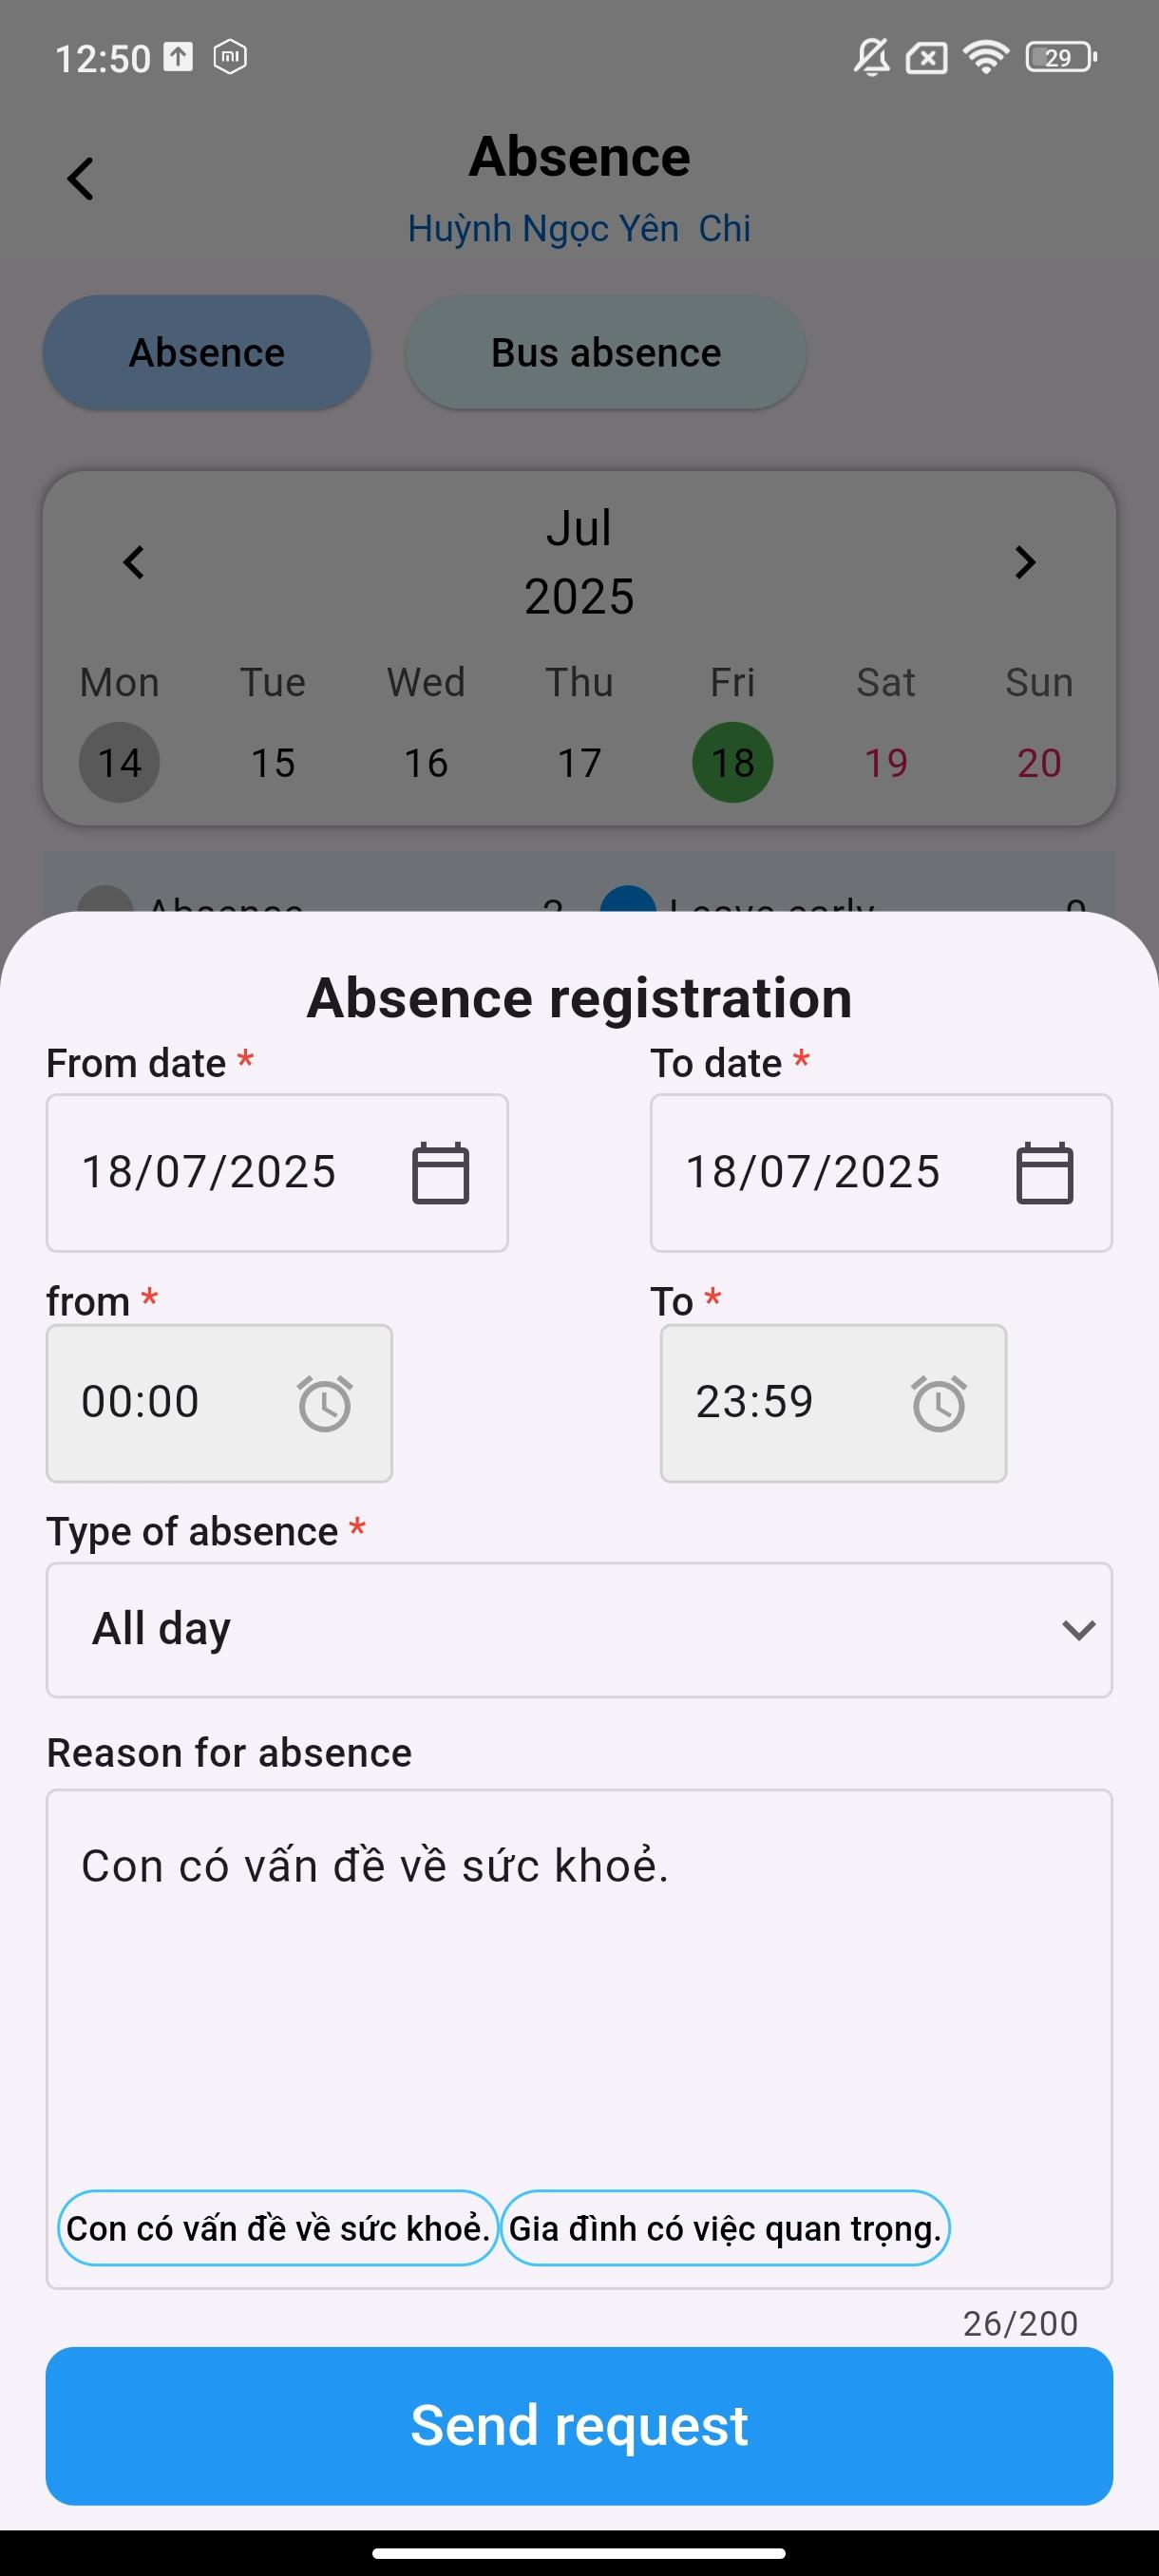
\includegraphics[width=0.6\textwidth]{images/create_leave_request_parent.png}
        \caption{Leave Request - Parent View}
        \label{subfig:leave_request_parent_view}
    \end{subfigure}
    \hfill
    \begin{subfigure}{0.45\textwidth}
        \centering
        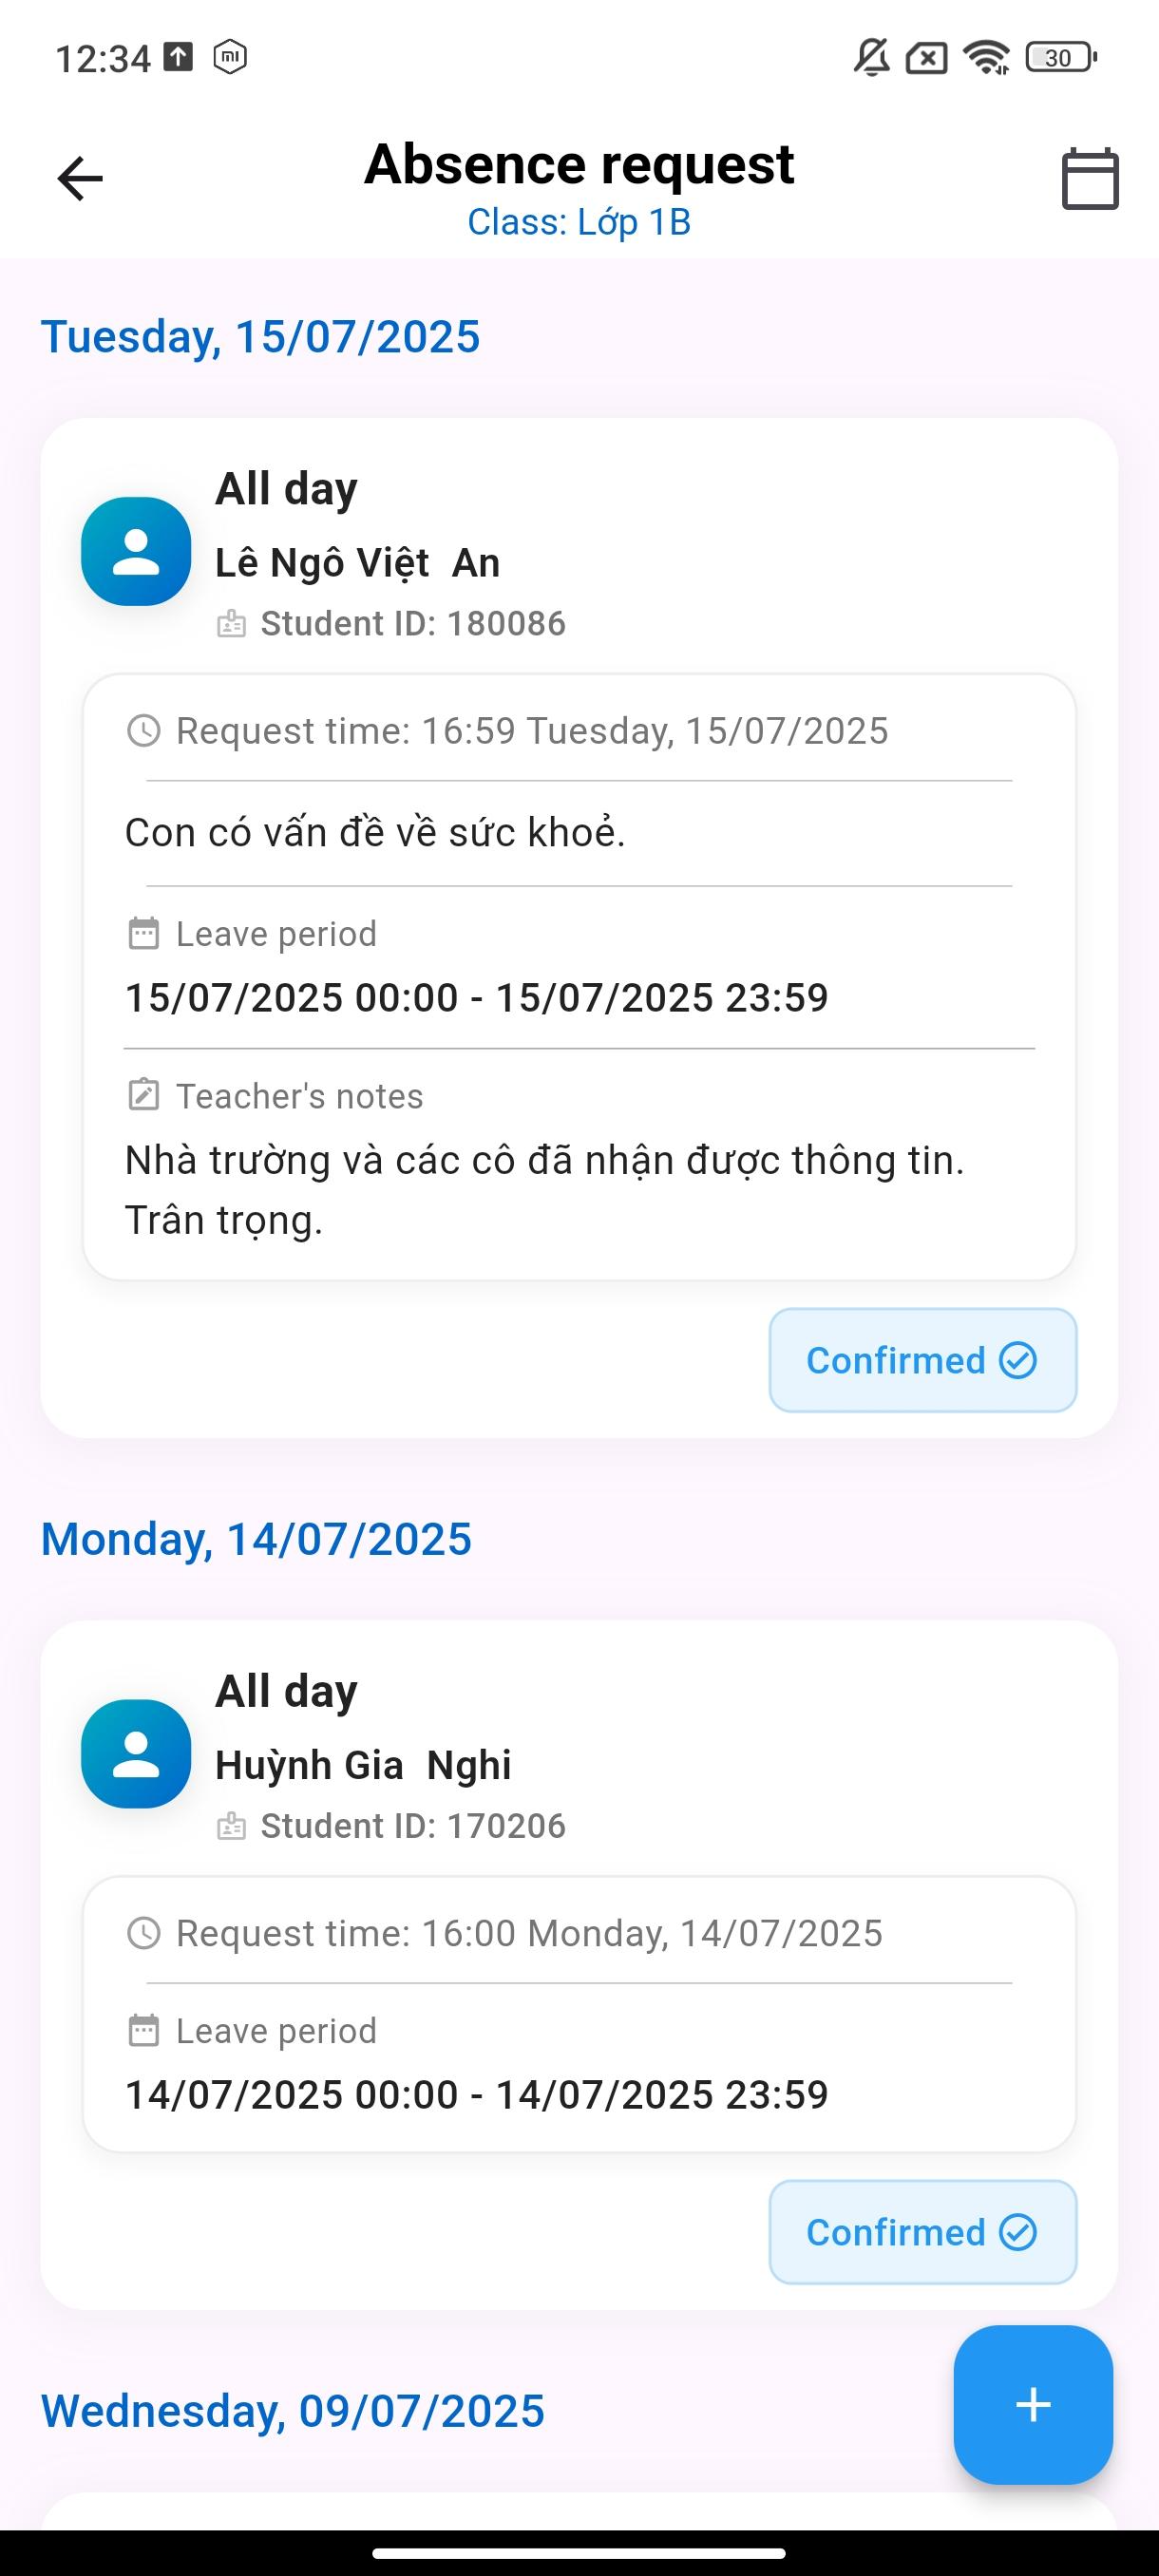
\includegraphics[width=0.6\textwidth]{images/approve_leave_request_teacher.png}
        \caption{Approve Leave - Teacher View}
        \label{subfig:create_leave_request_parent}
    \end{subfigure}
    \caption{Leave Request mobile app}
    \label{fig:leave_request_parent}
    \end{figure}
    %-------------------
    \newpage
    \item \textbf{Newsfeed Management}
    \begin{figure}[H]
    \centering
    \begin{subfigure}{0.45\textwidth}
        \centering
        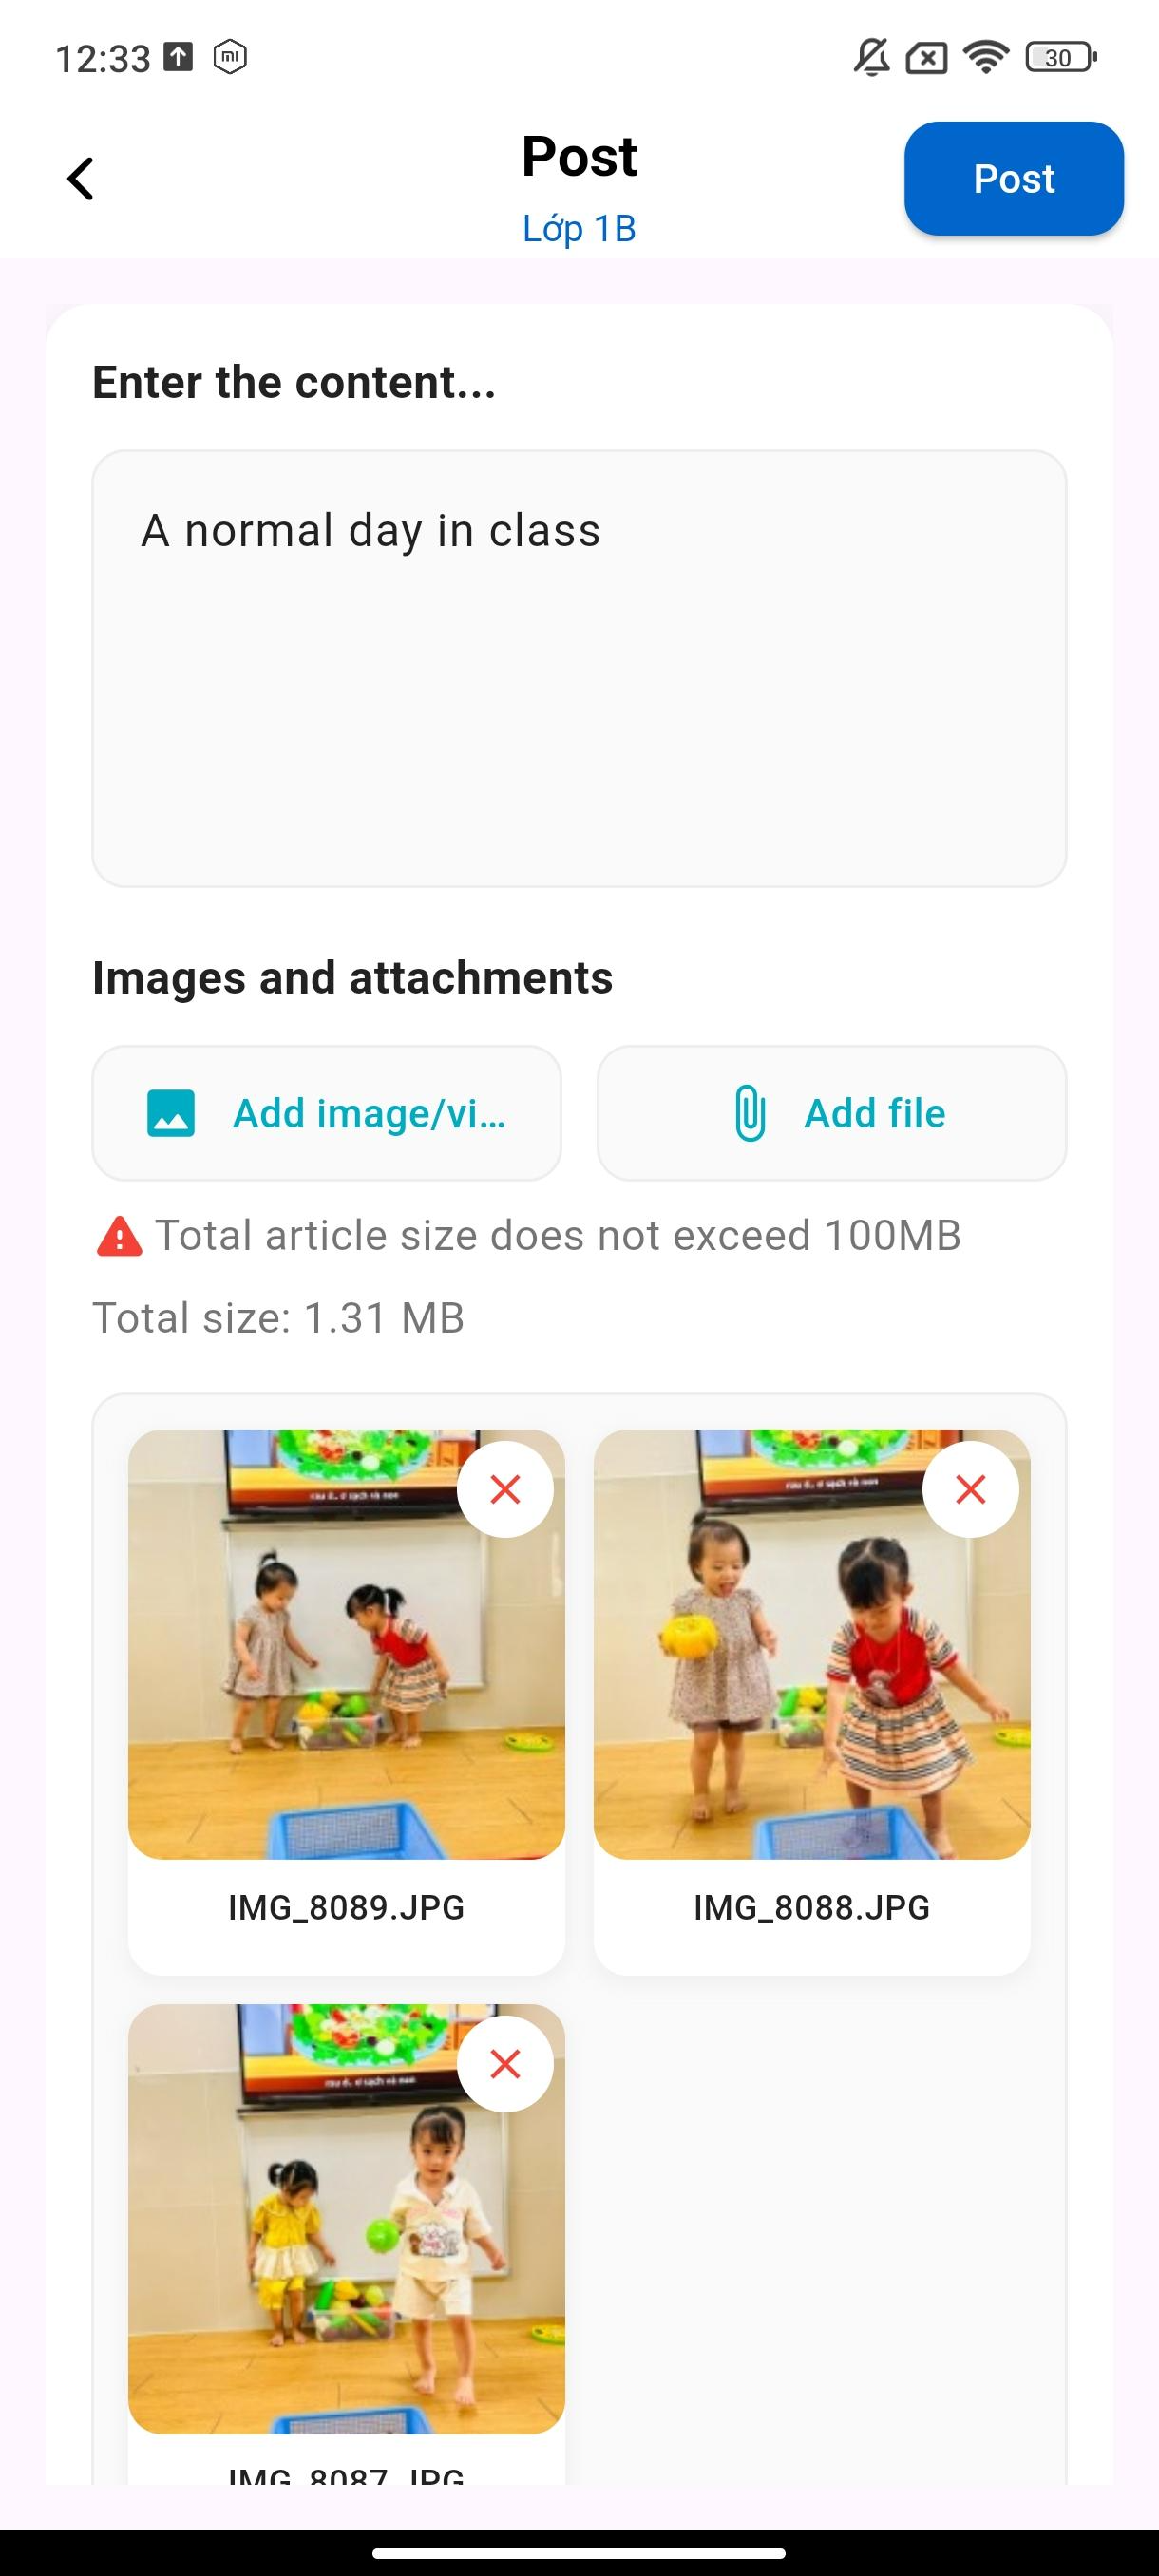
\includegraphics[width=0.6\textwidth]{images/create_post_teacher.png}
        \caption{Create Post Teacher View}
        \label{subfig:create_post_teacher_view}
    \end{subfigure}
    \hfill
    \begin{subfigure}{0.45\textwidth}
        \centering
        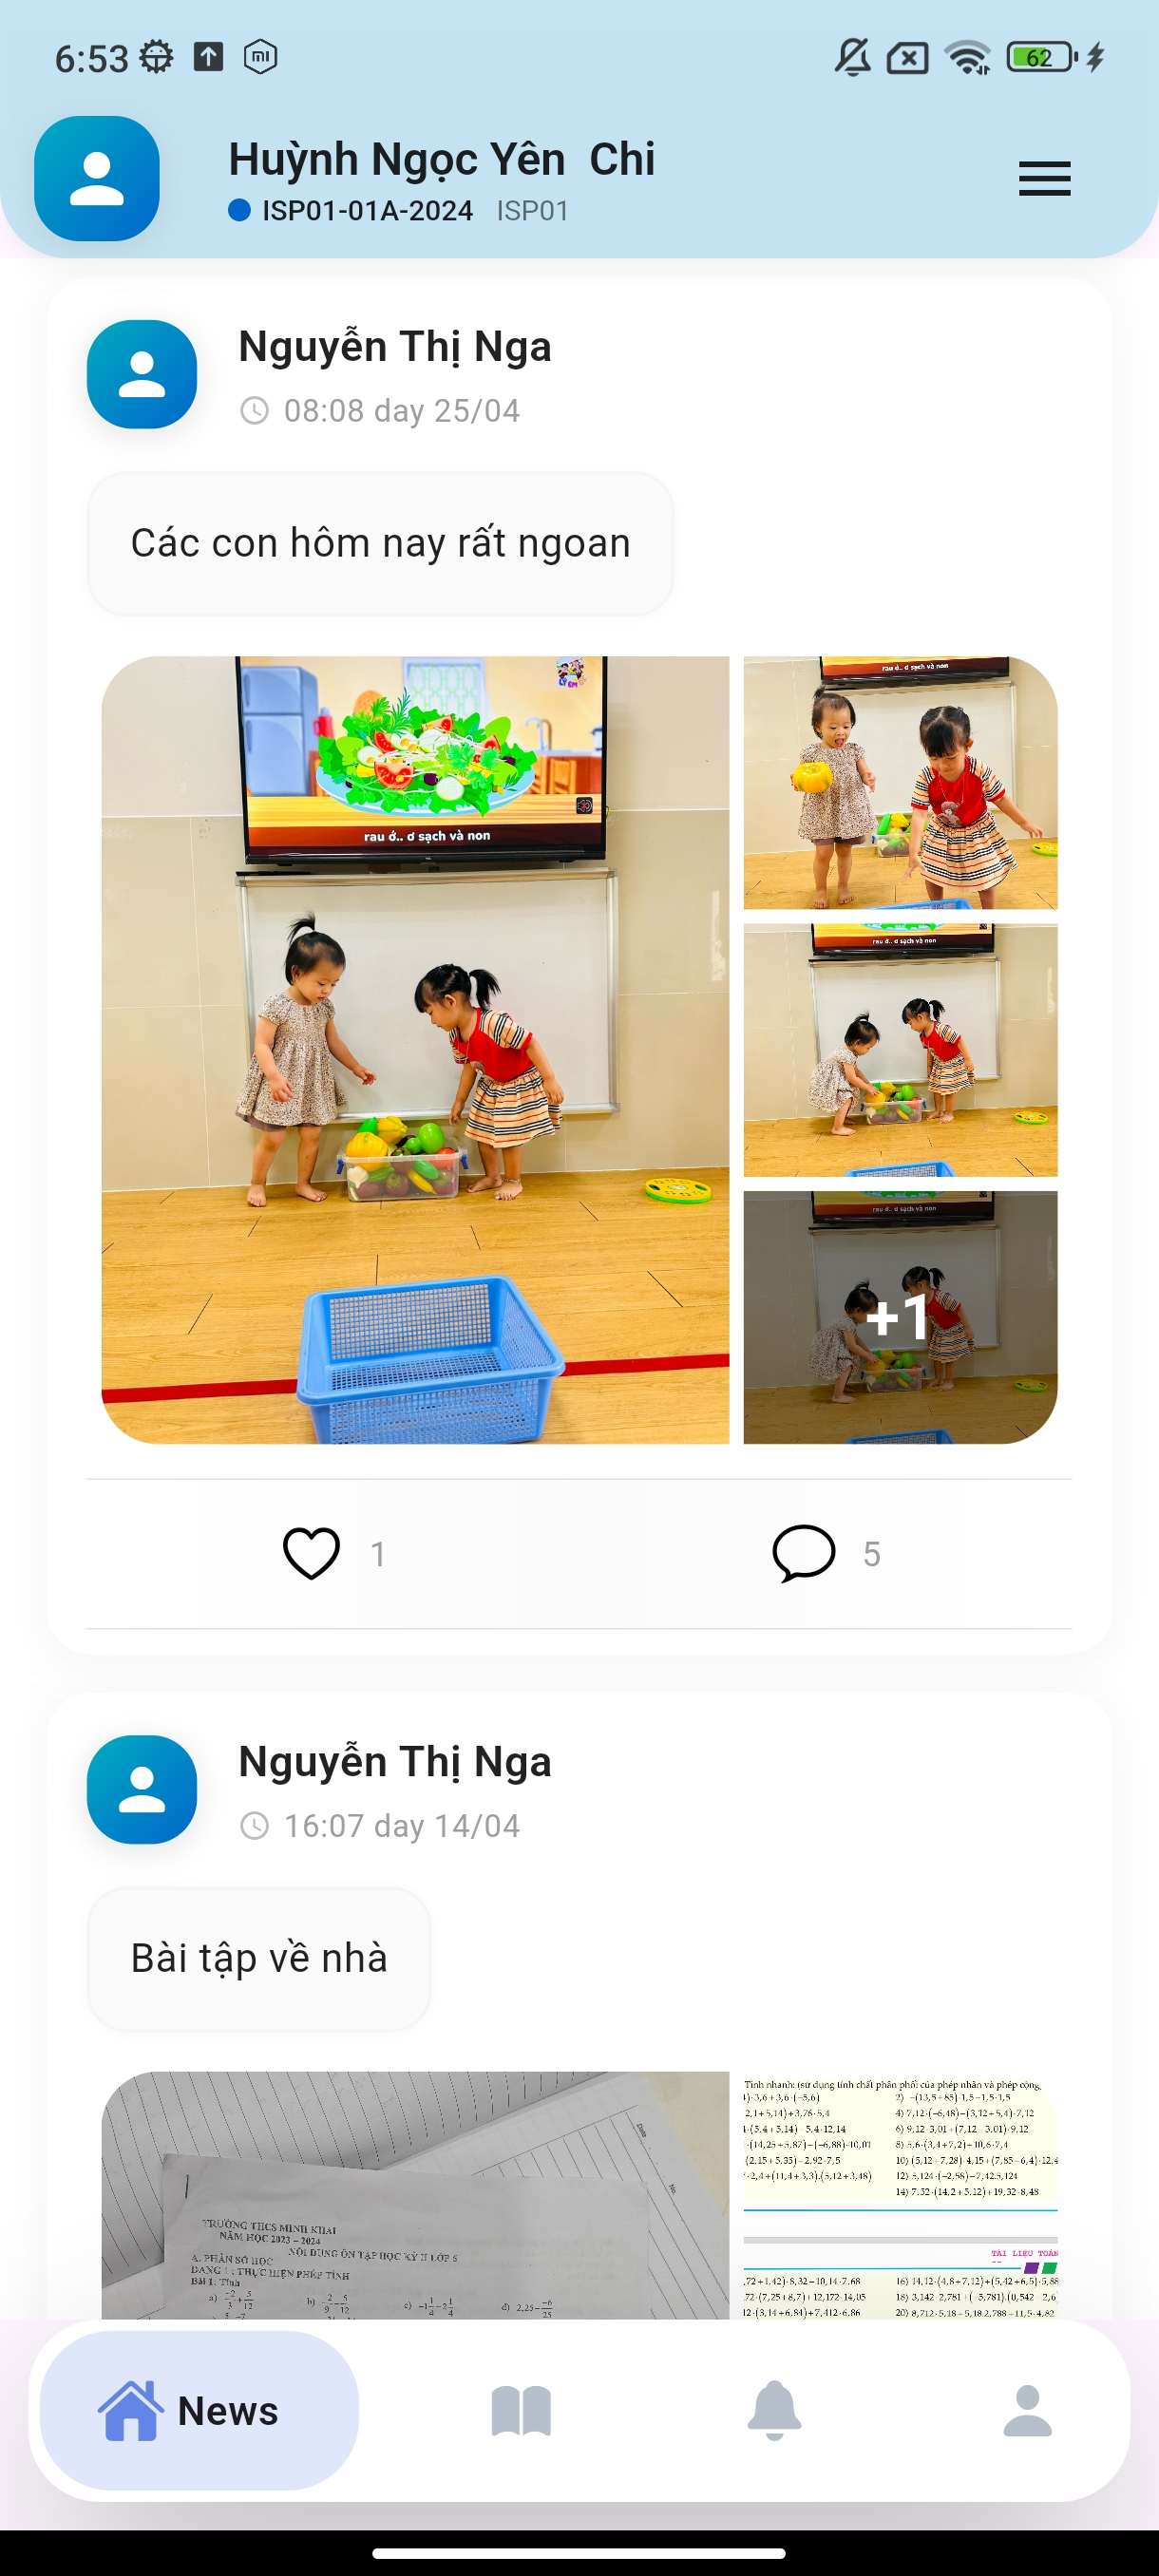
\includegraphics[width=0.6\textwidth]{images/appendix_news_student_mobile}
        \caption{Newsfeed Parent View}
        \label{subfig:newsfeed_parent_view}
    \end{subfigure}
    \caption{Newsfeed mobile app}
    \label{fig:newsfeed_mobile_app}
    \end{figure}
    %--------------
    \item \textbf{Student Attendance Management}
    \begin{figure}[H]
    \centering
    \begin{subfigure}{0.45\textwidth}
        \centering
        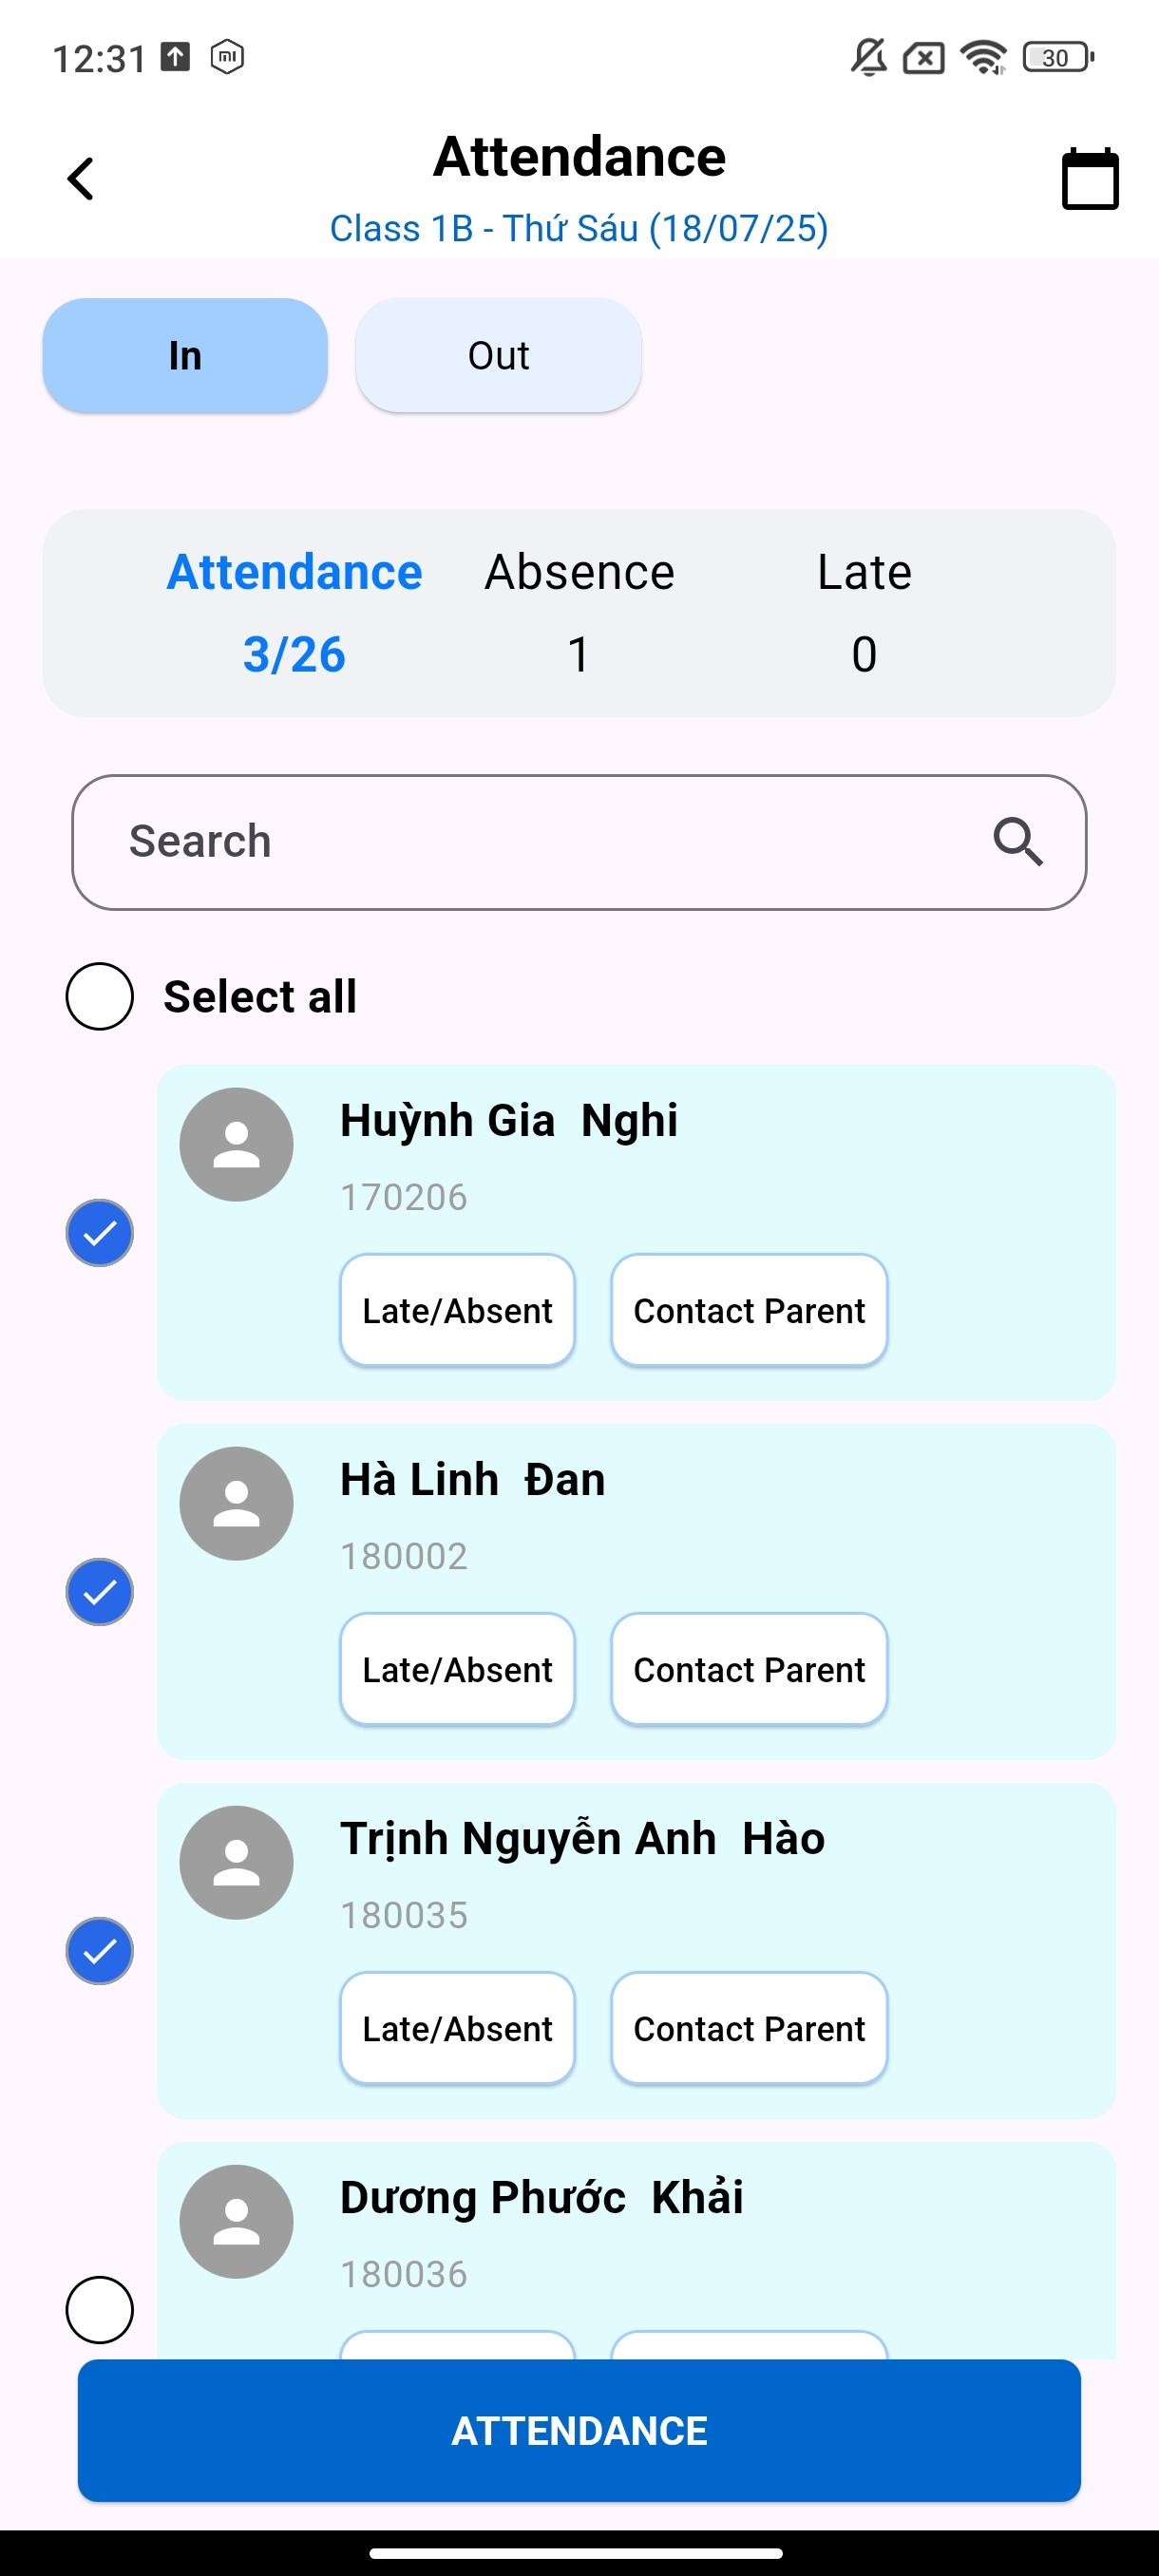
\includegraphics[width=0.6\textwidth]{images/attendance_teacher_view.png}
        \caption{Attendance - Teacher View}
        \label{subfig:attendance_teacher_view}
    \end{subfigure}
    \hfill
    \begin{subfigure}{0.45\textwidth}
        \centering
        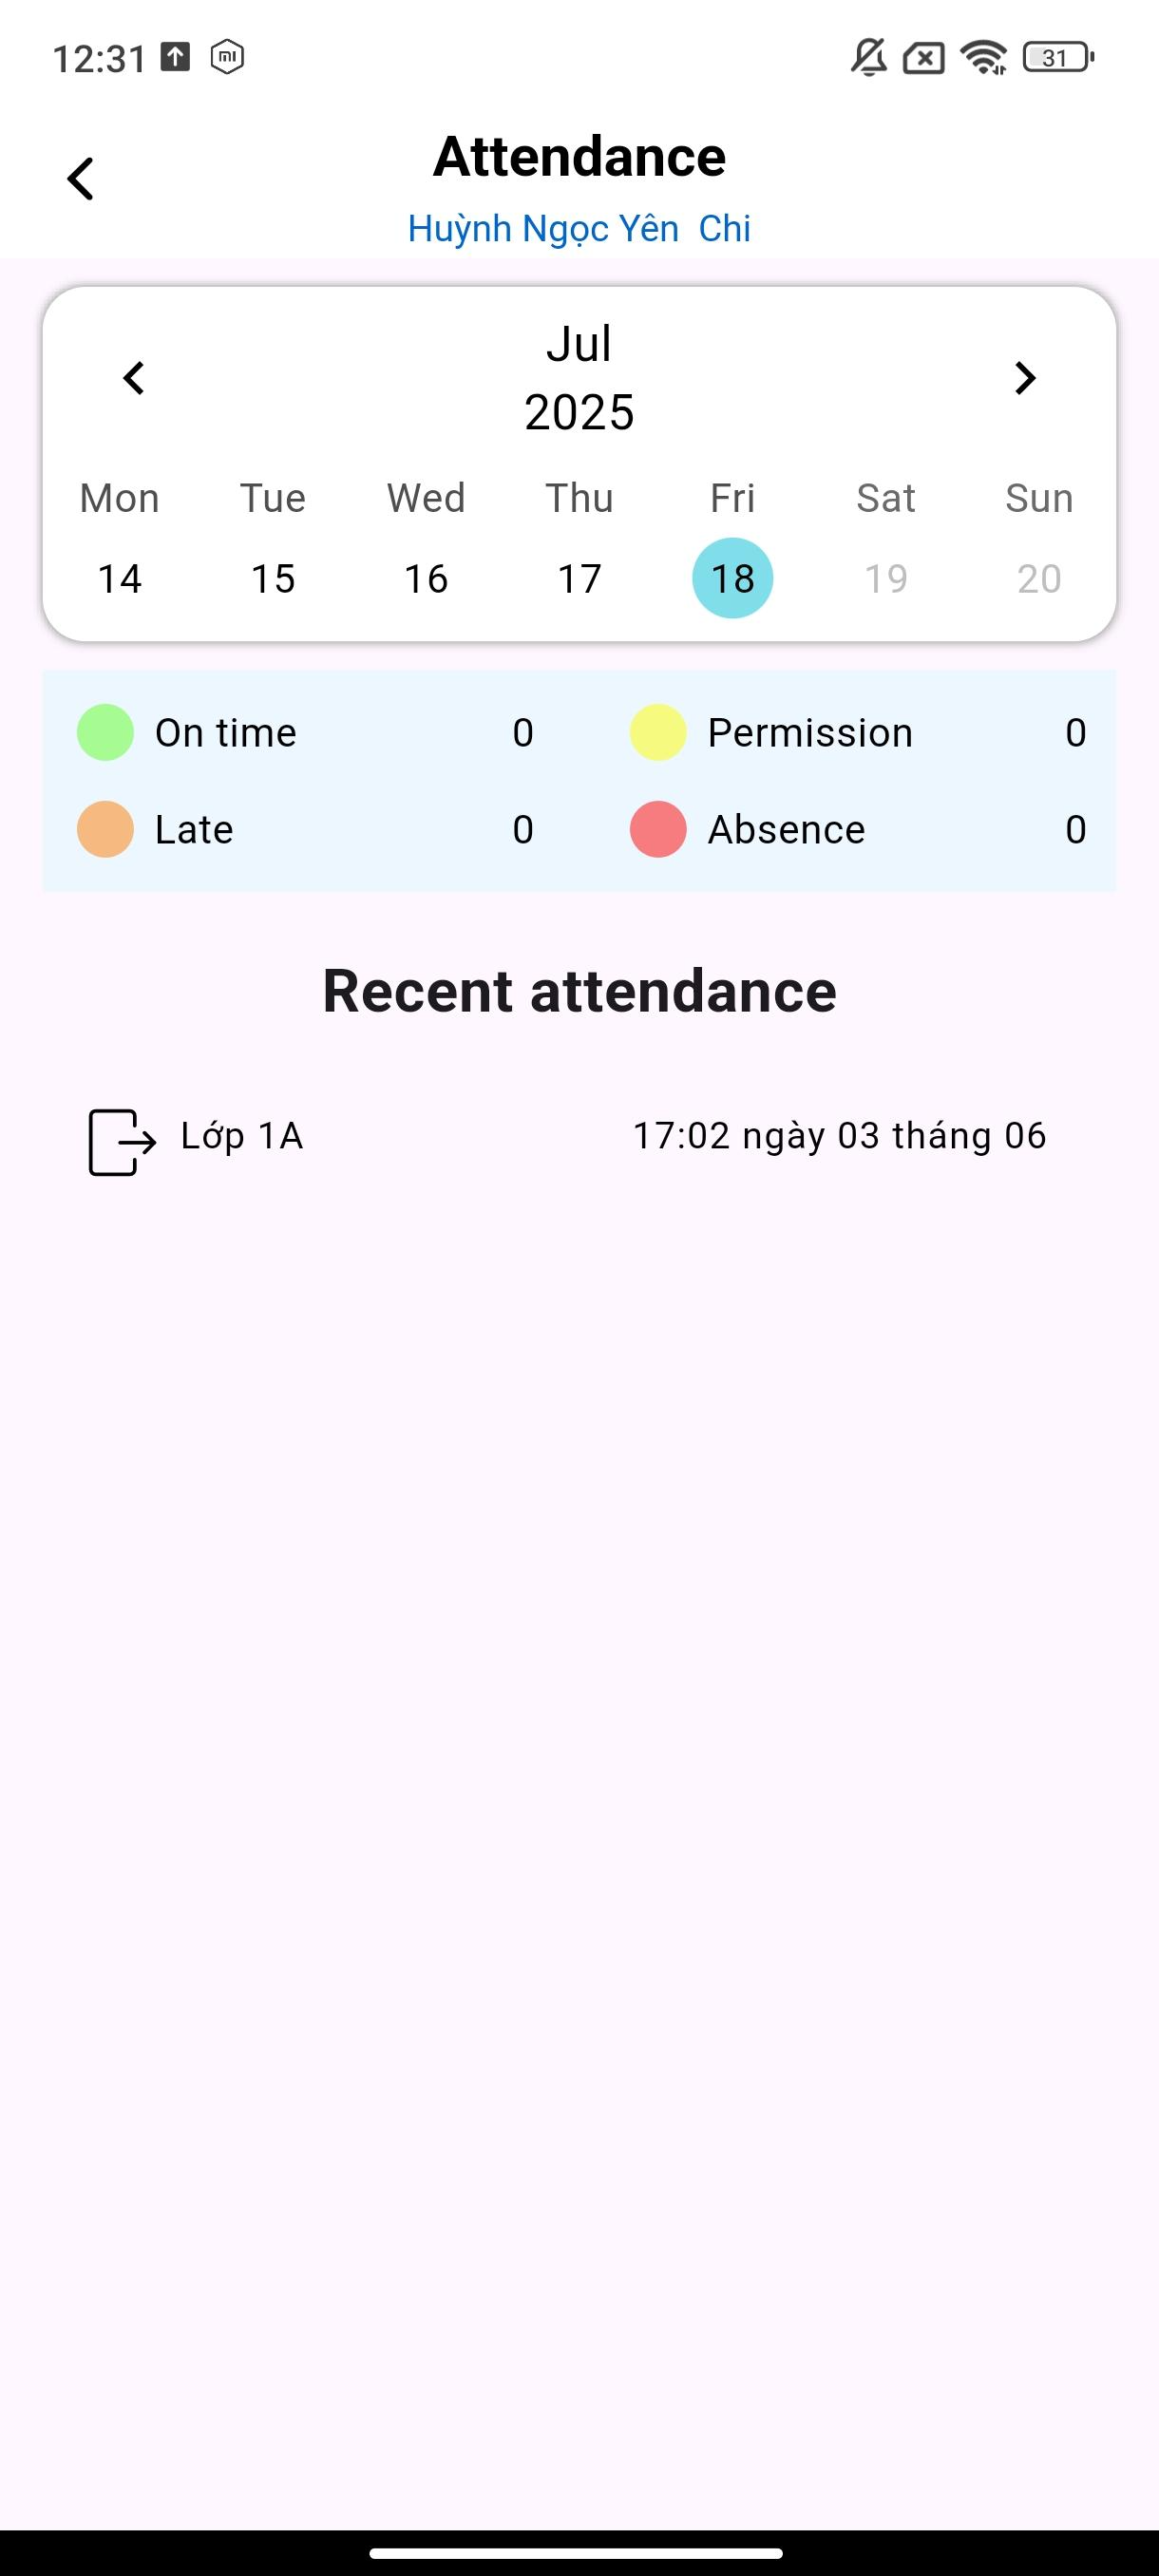
\includegraphics[width=0.6\textwidth]{images/attendance_parent_view.png}
        \caption{Attendance - Parent View}
        \label{subfig:attendance_parent_view}
    \end{subfigure}
    \caption{Attendance mobile app}
    \label{fig:attendance_mobile_app}
    \end{figure}
    \begin{figure}[H]
    \centering
    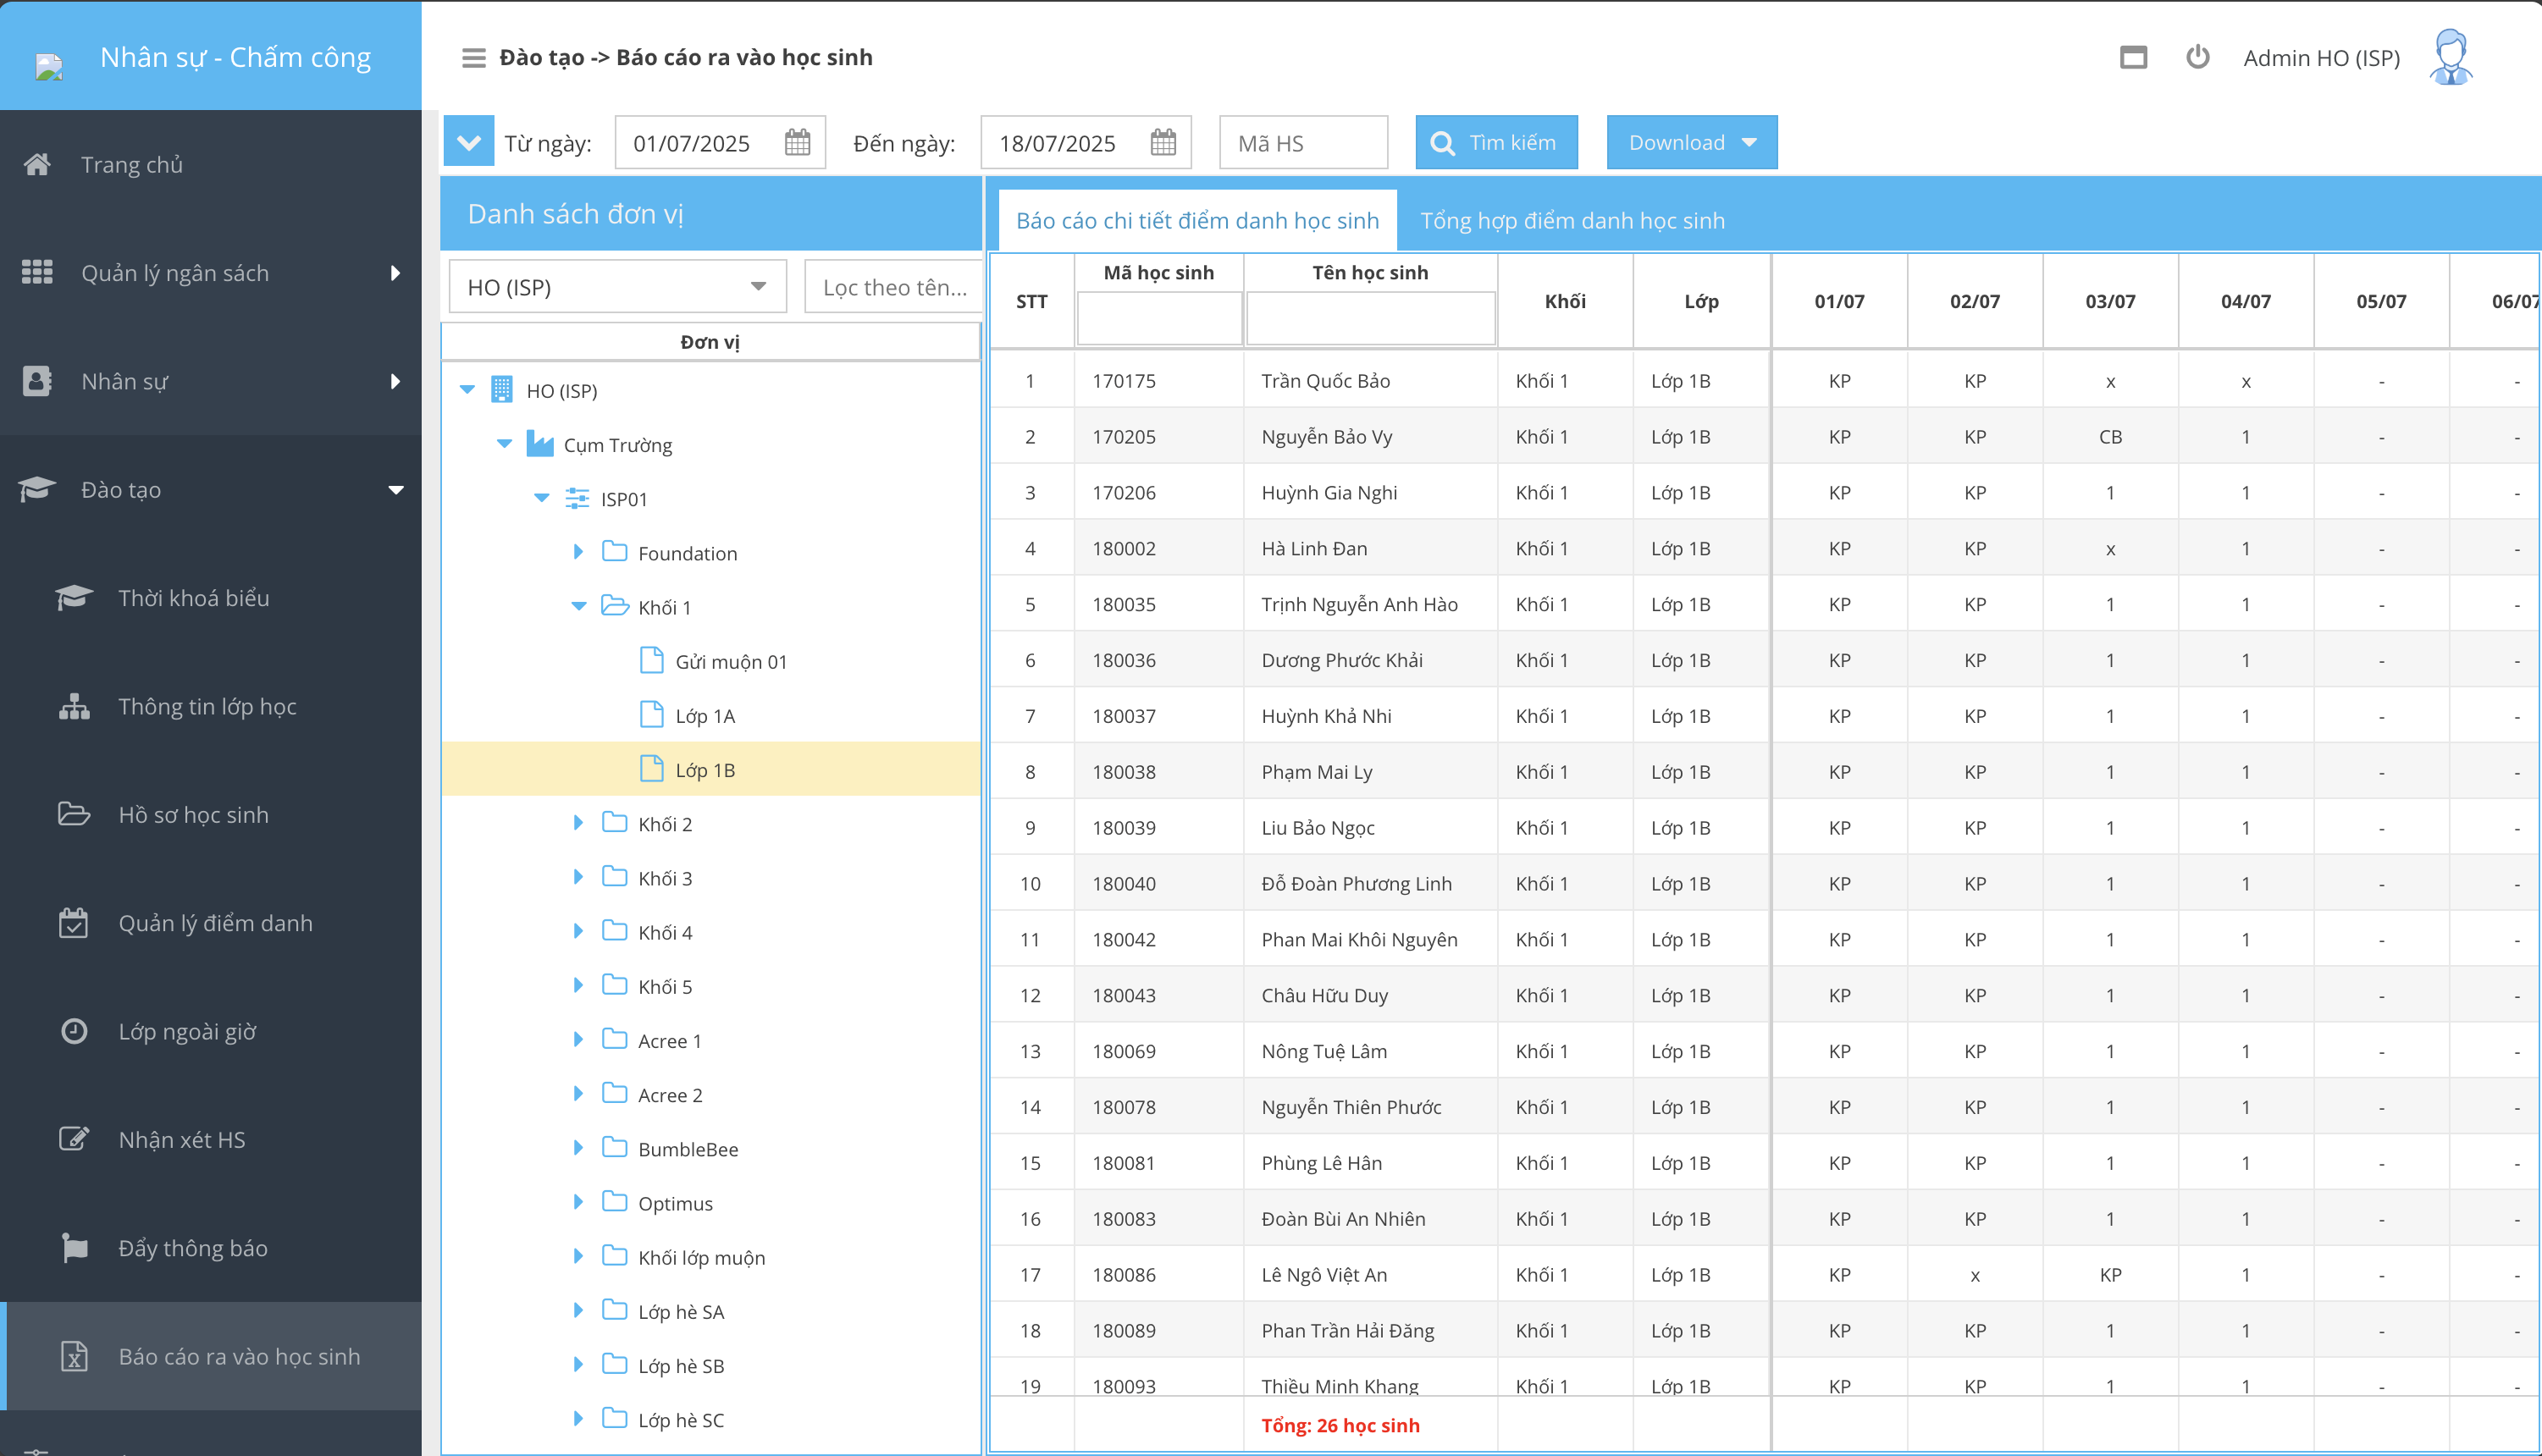
\includegraphics[width=1\textwidth]{images/student_attendance_report.png}
    \vspace{-1em}
    \caption{Student attendance report web app.}
    \label{fig:attendance_report_web}
    \end{figure}
    %--------------
    \item \textbf{Student Assessments Management}
    \begin{figure}[H]
    \centering
    \begin{subfigure}{0.45\textwidth}
        \centering
        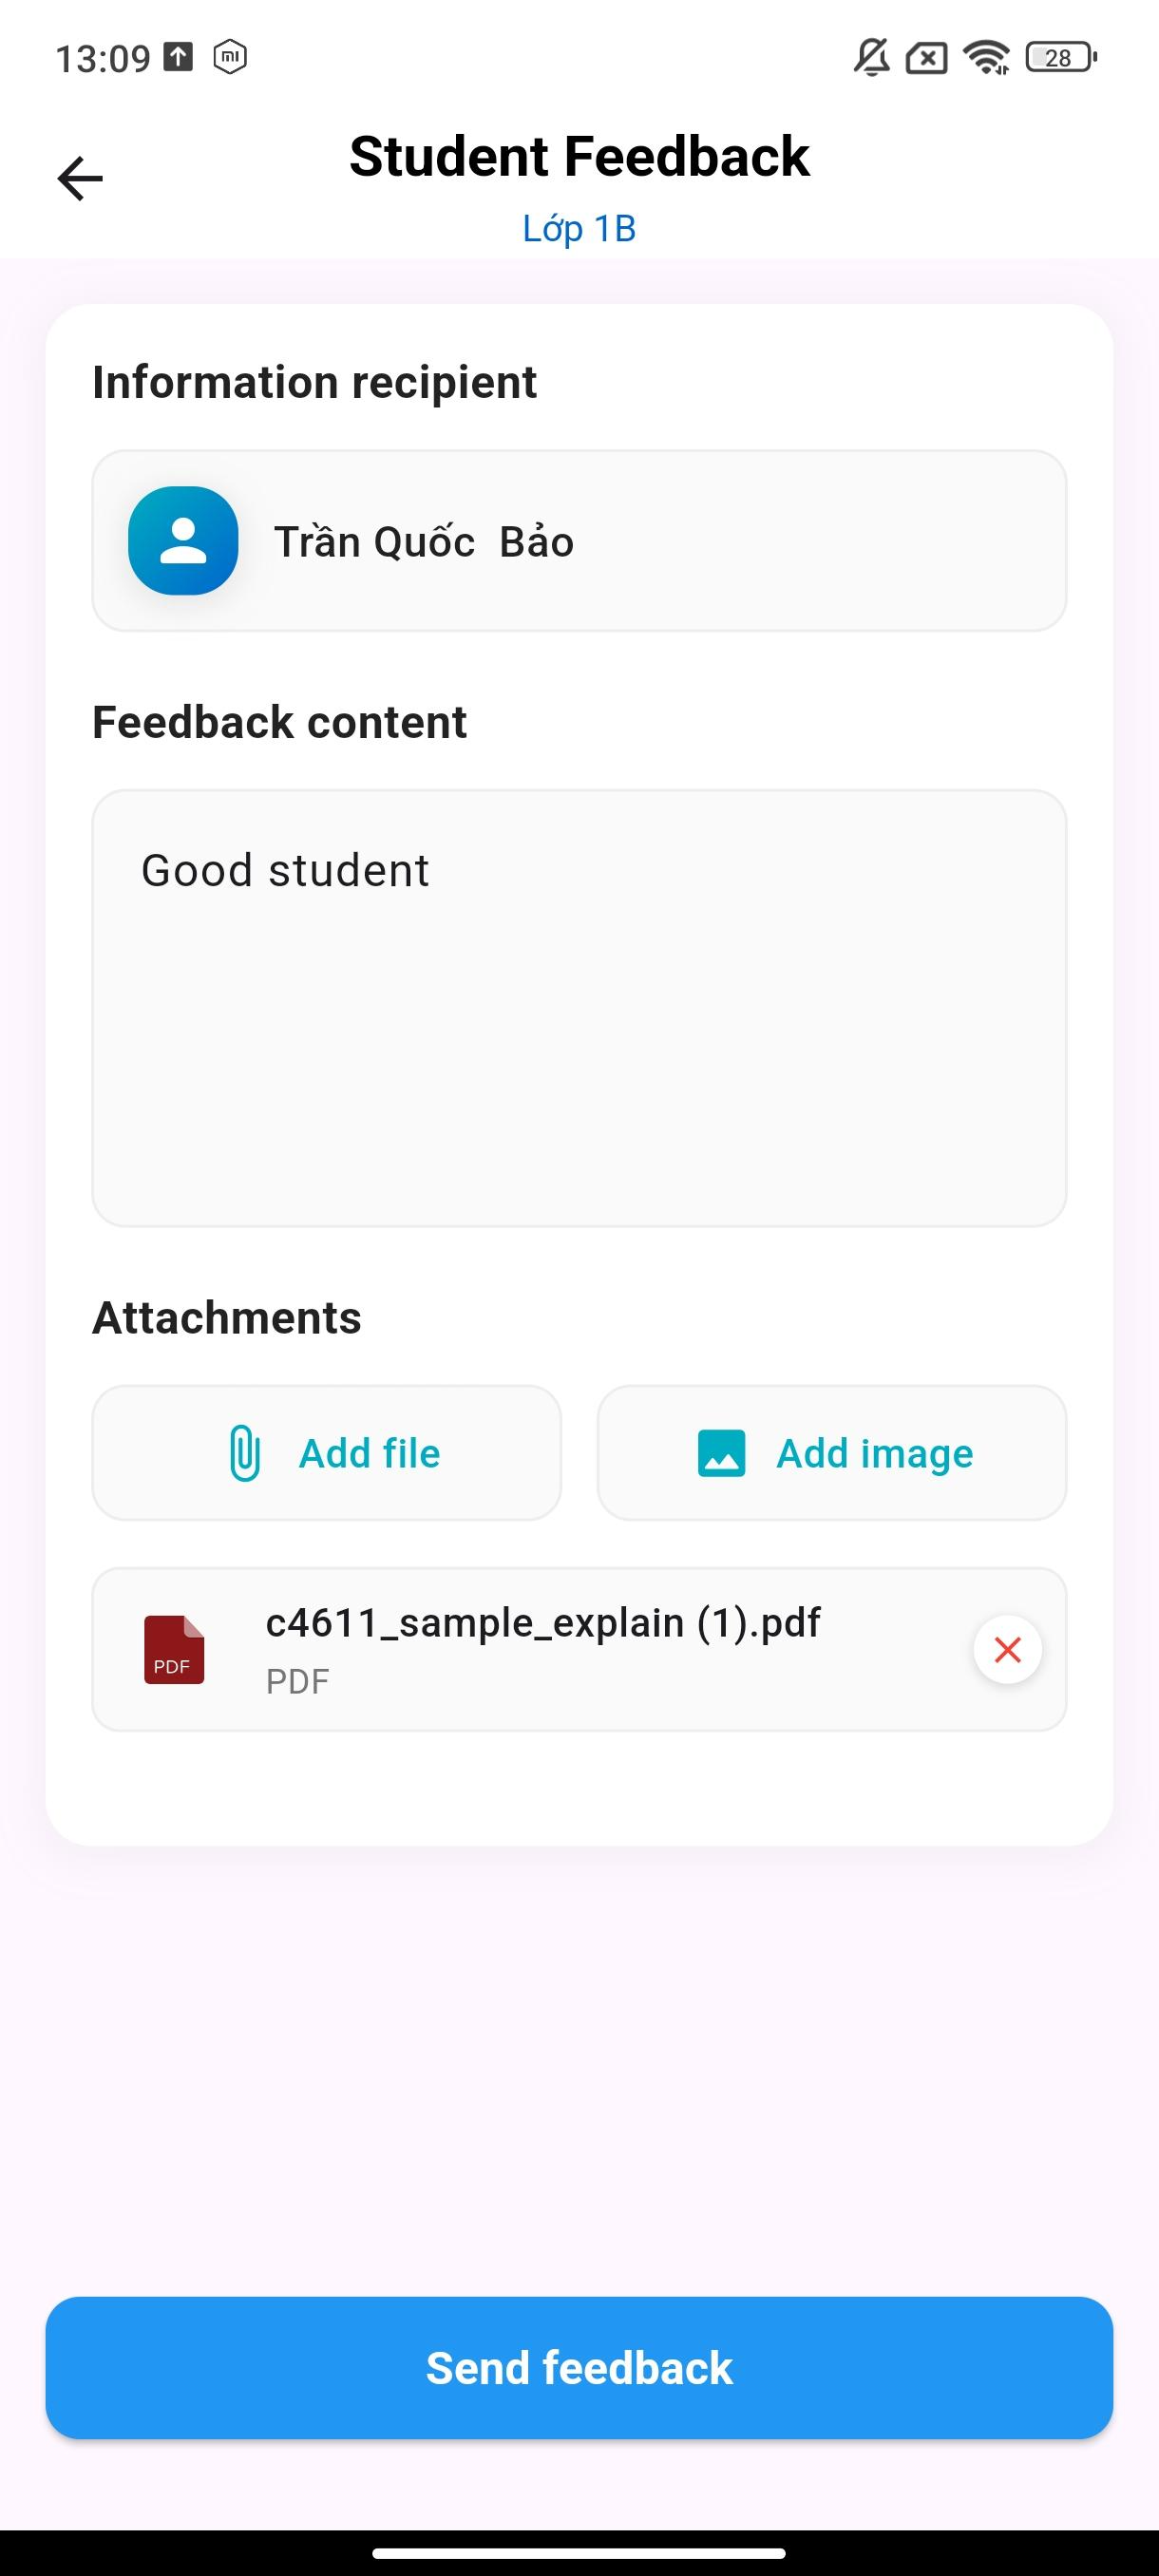
\includegraphics[width=0.6\textwidth]{images/assess_teacher_view.png}
        \caption{Assess Student - Teacher View}
        \label{subfig:assess_student_teacher_view}
    \end{subfigure}
    \hfill
    \begin{subfigure}{0.45\textwidth}
        \centering
        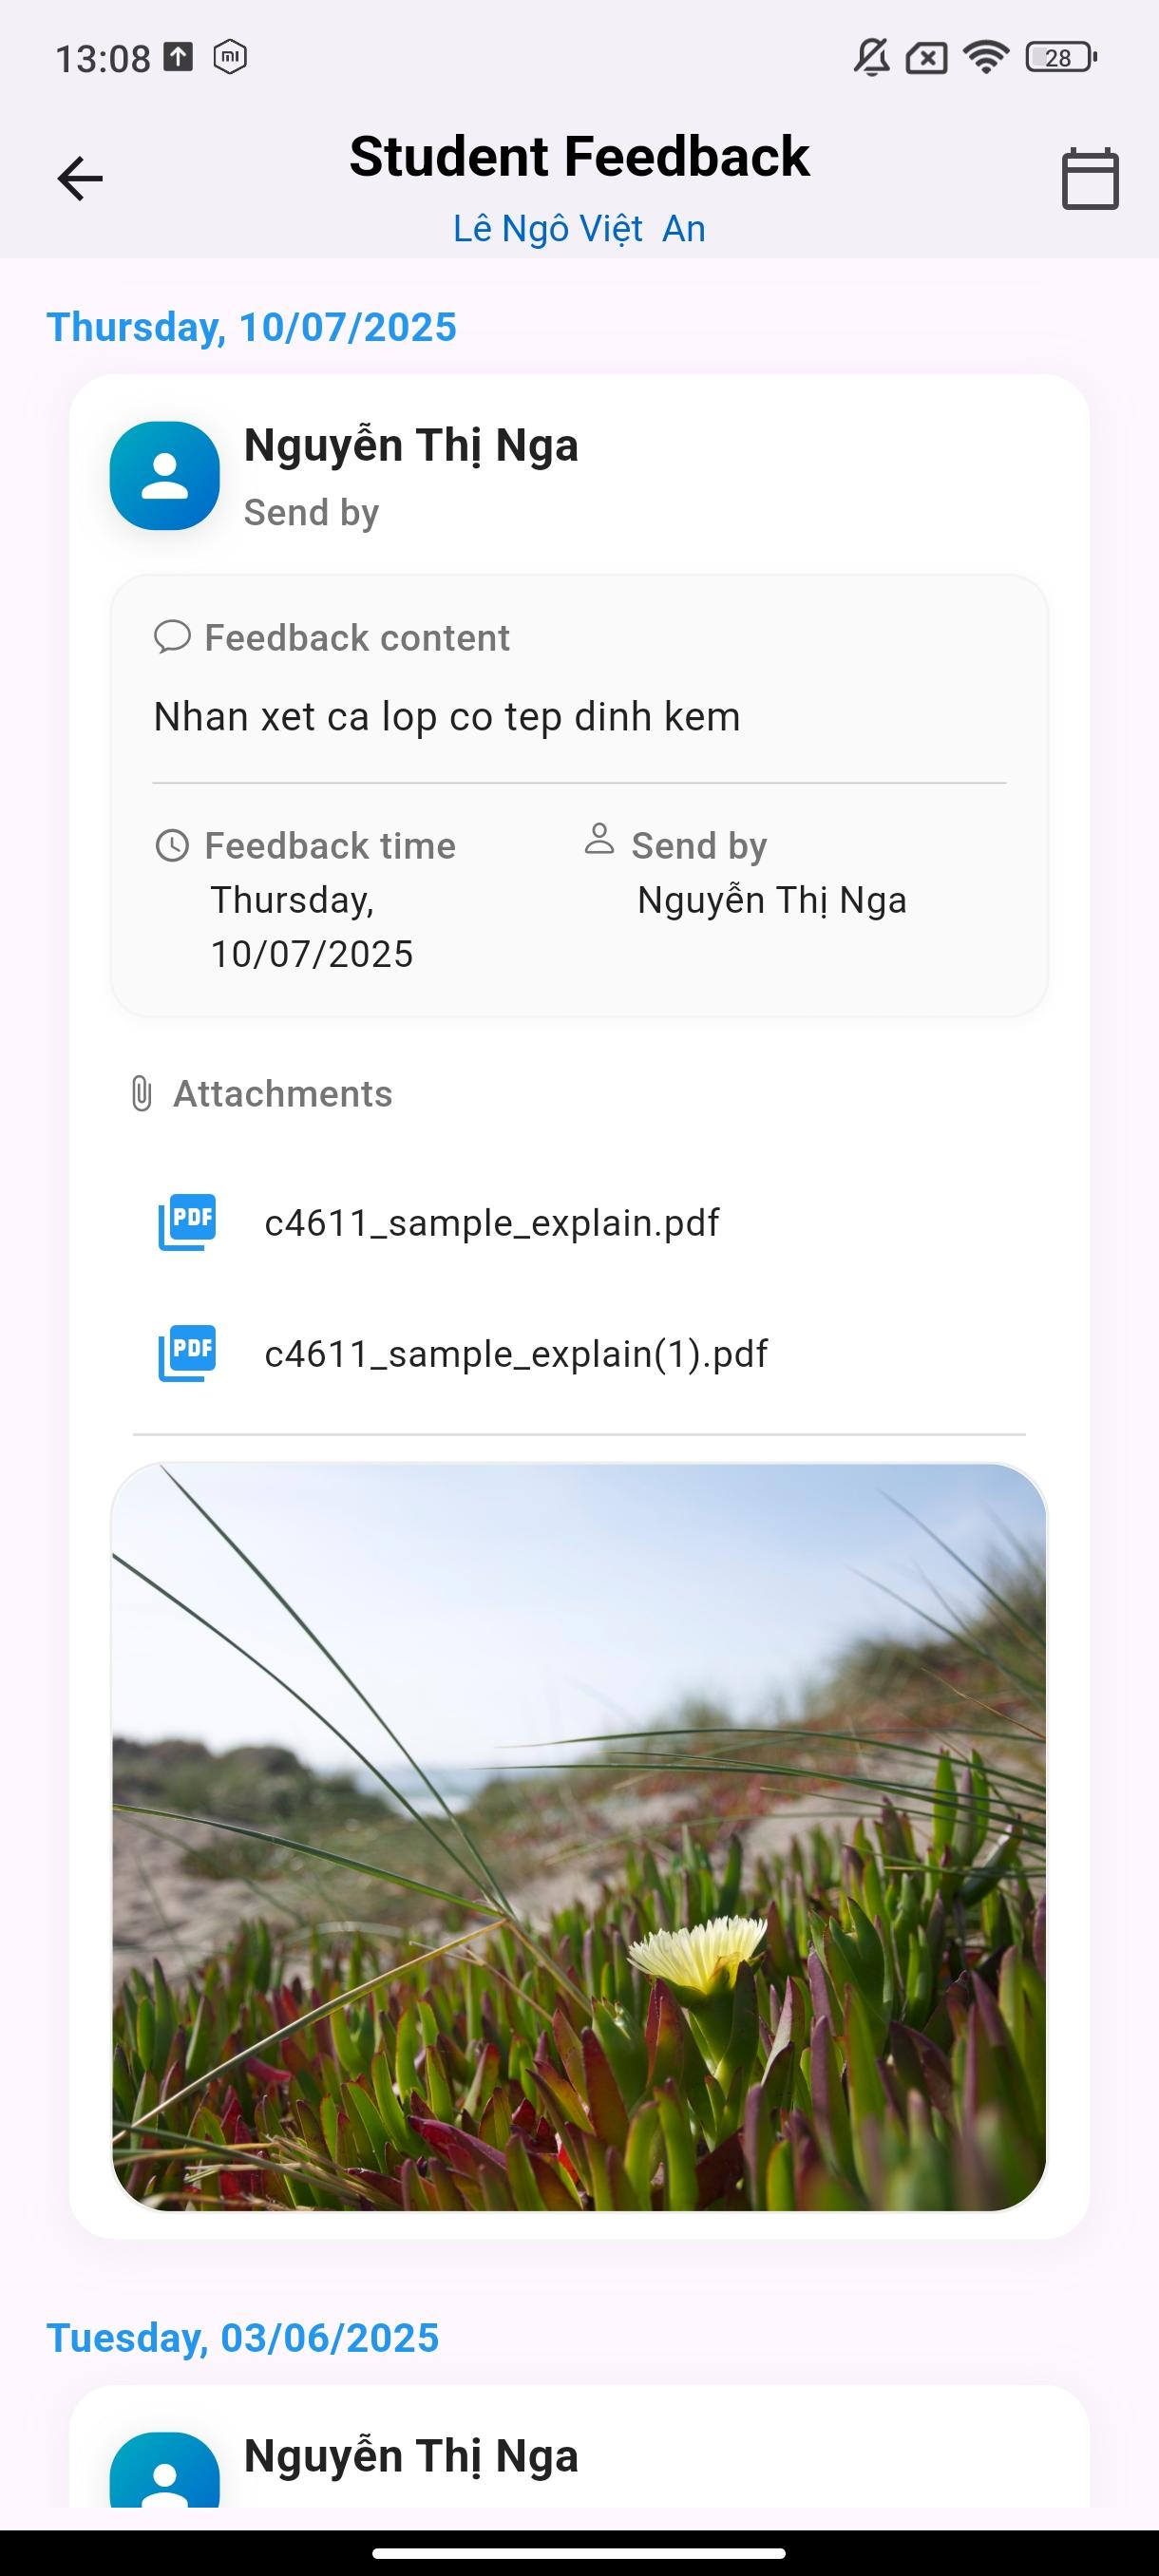
\includegraphics[width=0.6\textwidth]{images/assess_student_view.png}
        \caption{Assess Student - Parent View}
        \label{subfig:assess_student_parent_view}
    \end{subfigure}
    \caption{Assess Student mobile app}
    \label{fig:assess_student_mobile_app}
    \end{figure}
    %---------------------
    \newpage
    \item \textbf{Medicine Reminder Management}
    \begin{figure}[H]
    \centering
    \begin{subfigure}{0.45\textwidth}
        \centering
        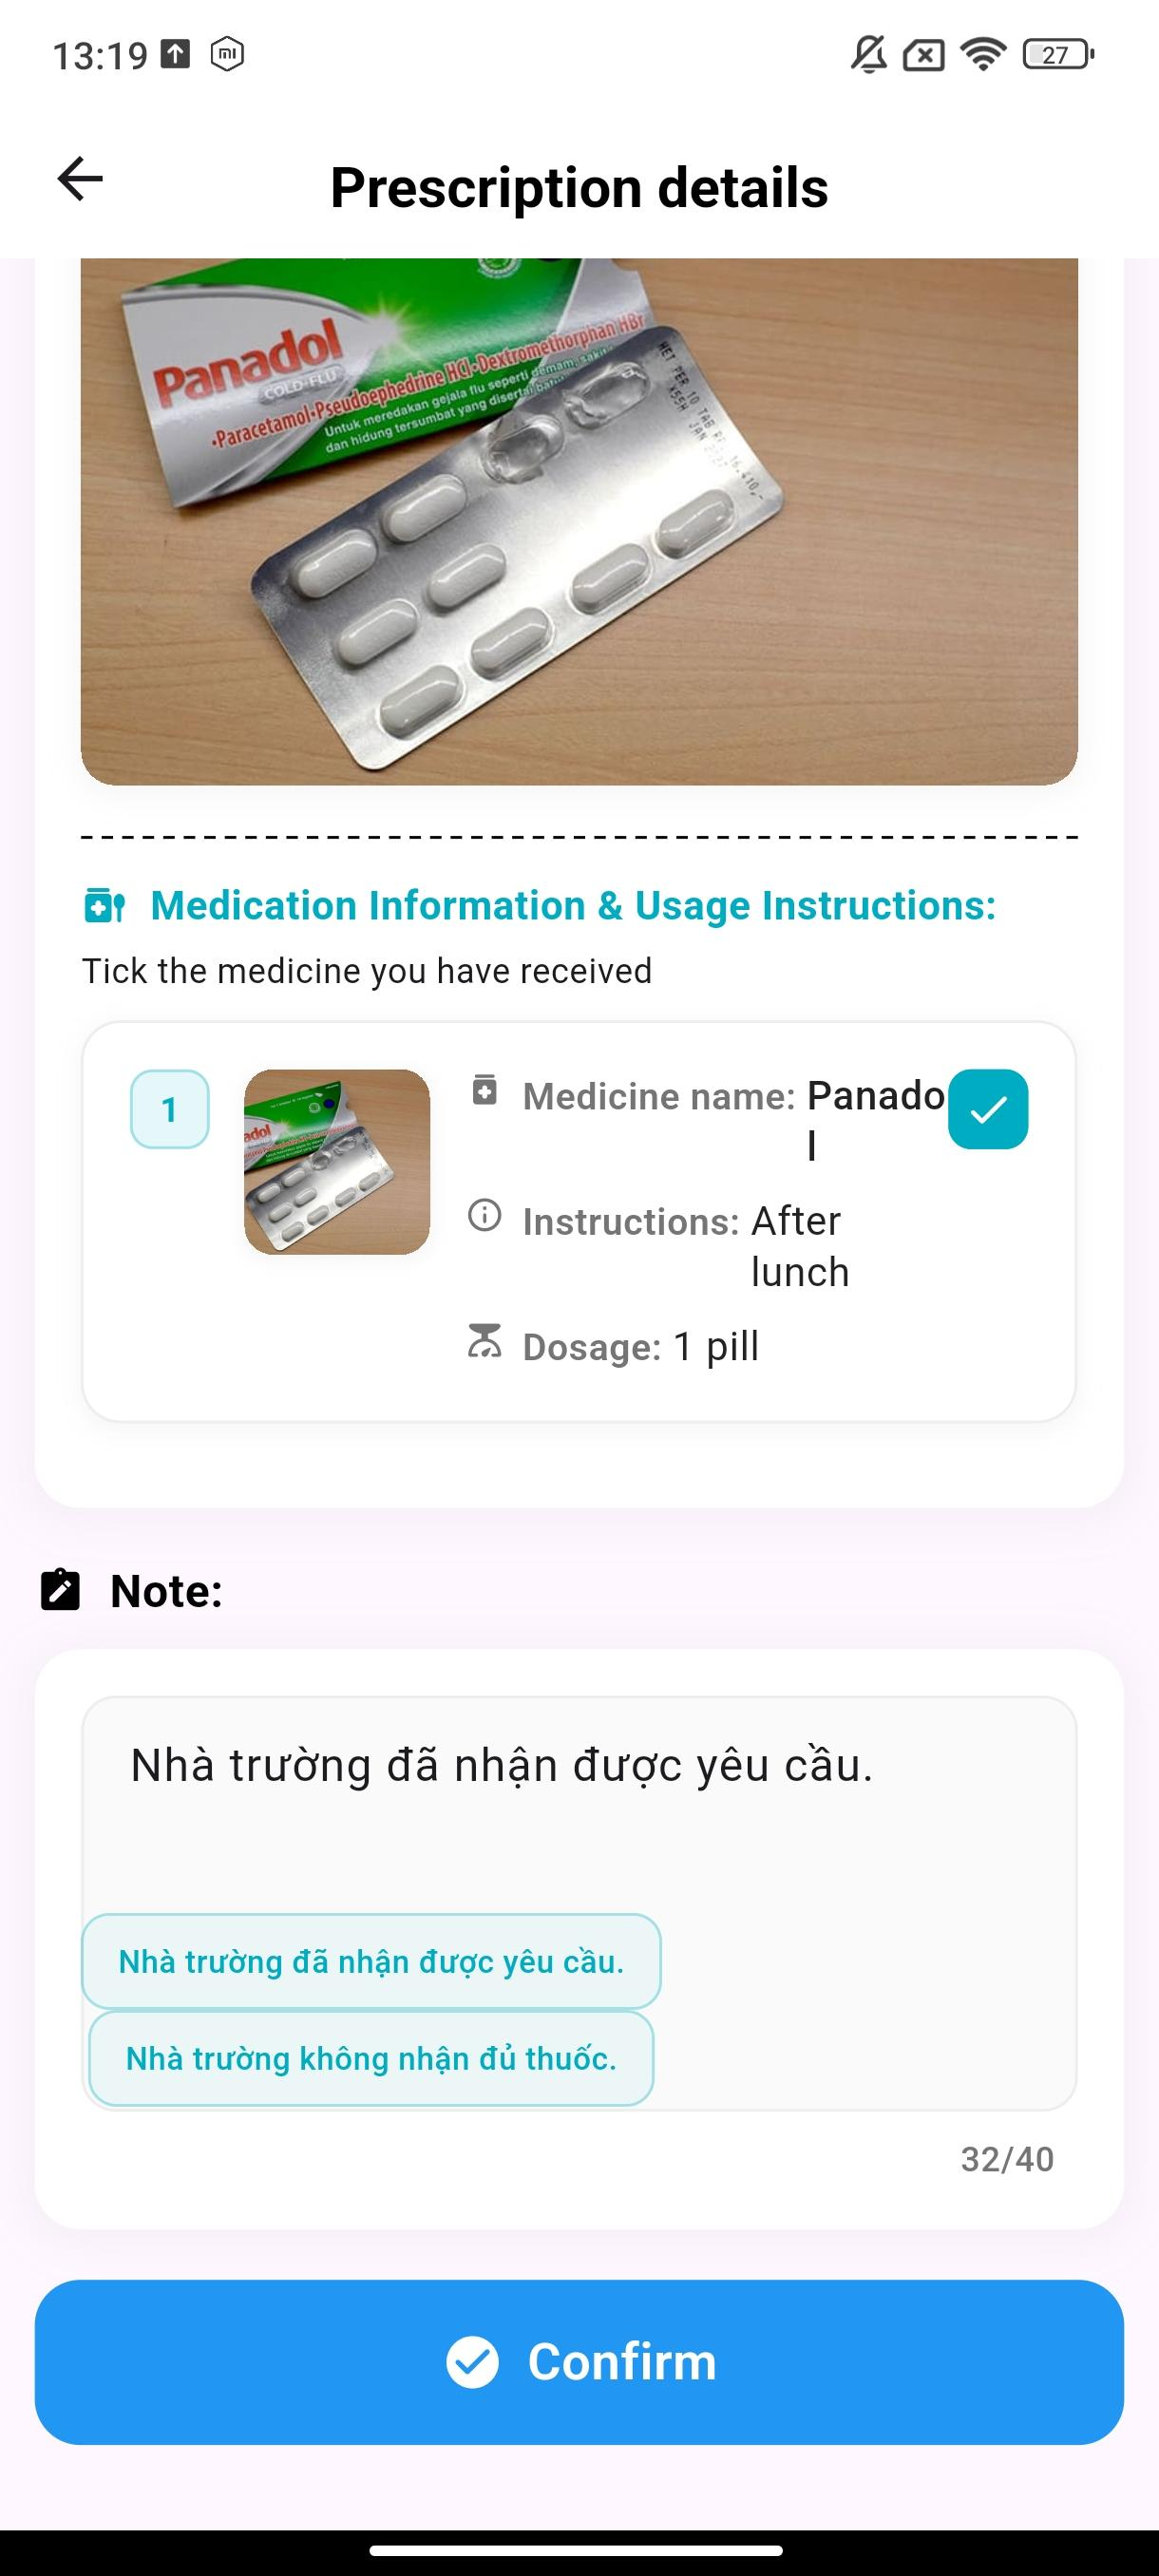
\includegraphics[width=0.6\textwidth]{images/medicine_reminder_confirmation_teacher.png}
        \caption{Medicine Reminder - Teacher Confimation View}
        \label{subfig:medicine_reminder_teacher_view}
    \end{subfigure}
    \hfill
    \begin{subfigure}{0.45\textwidth}
        \centering
        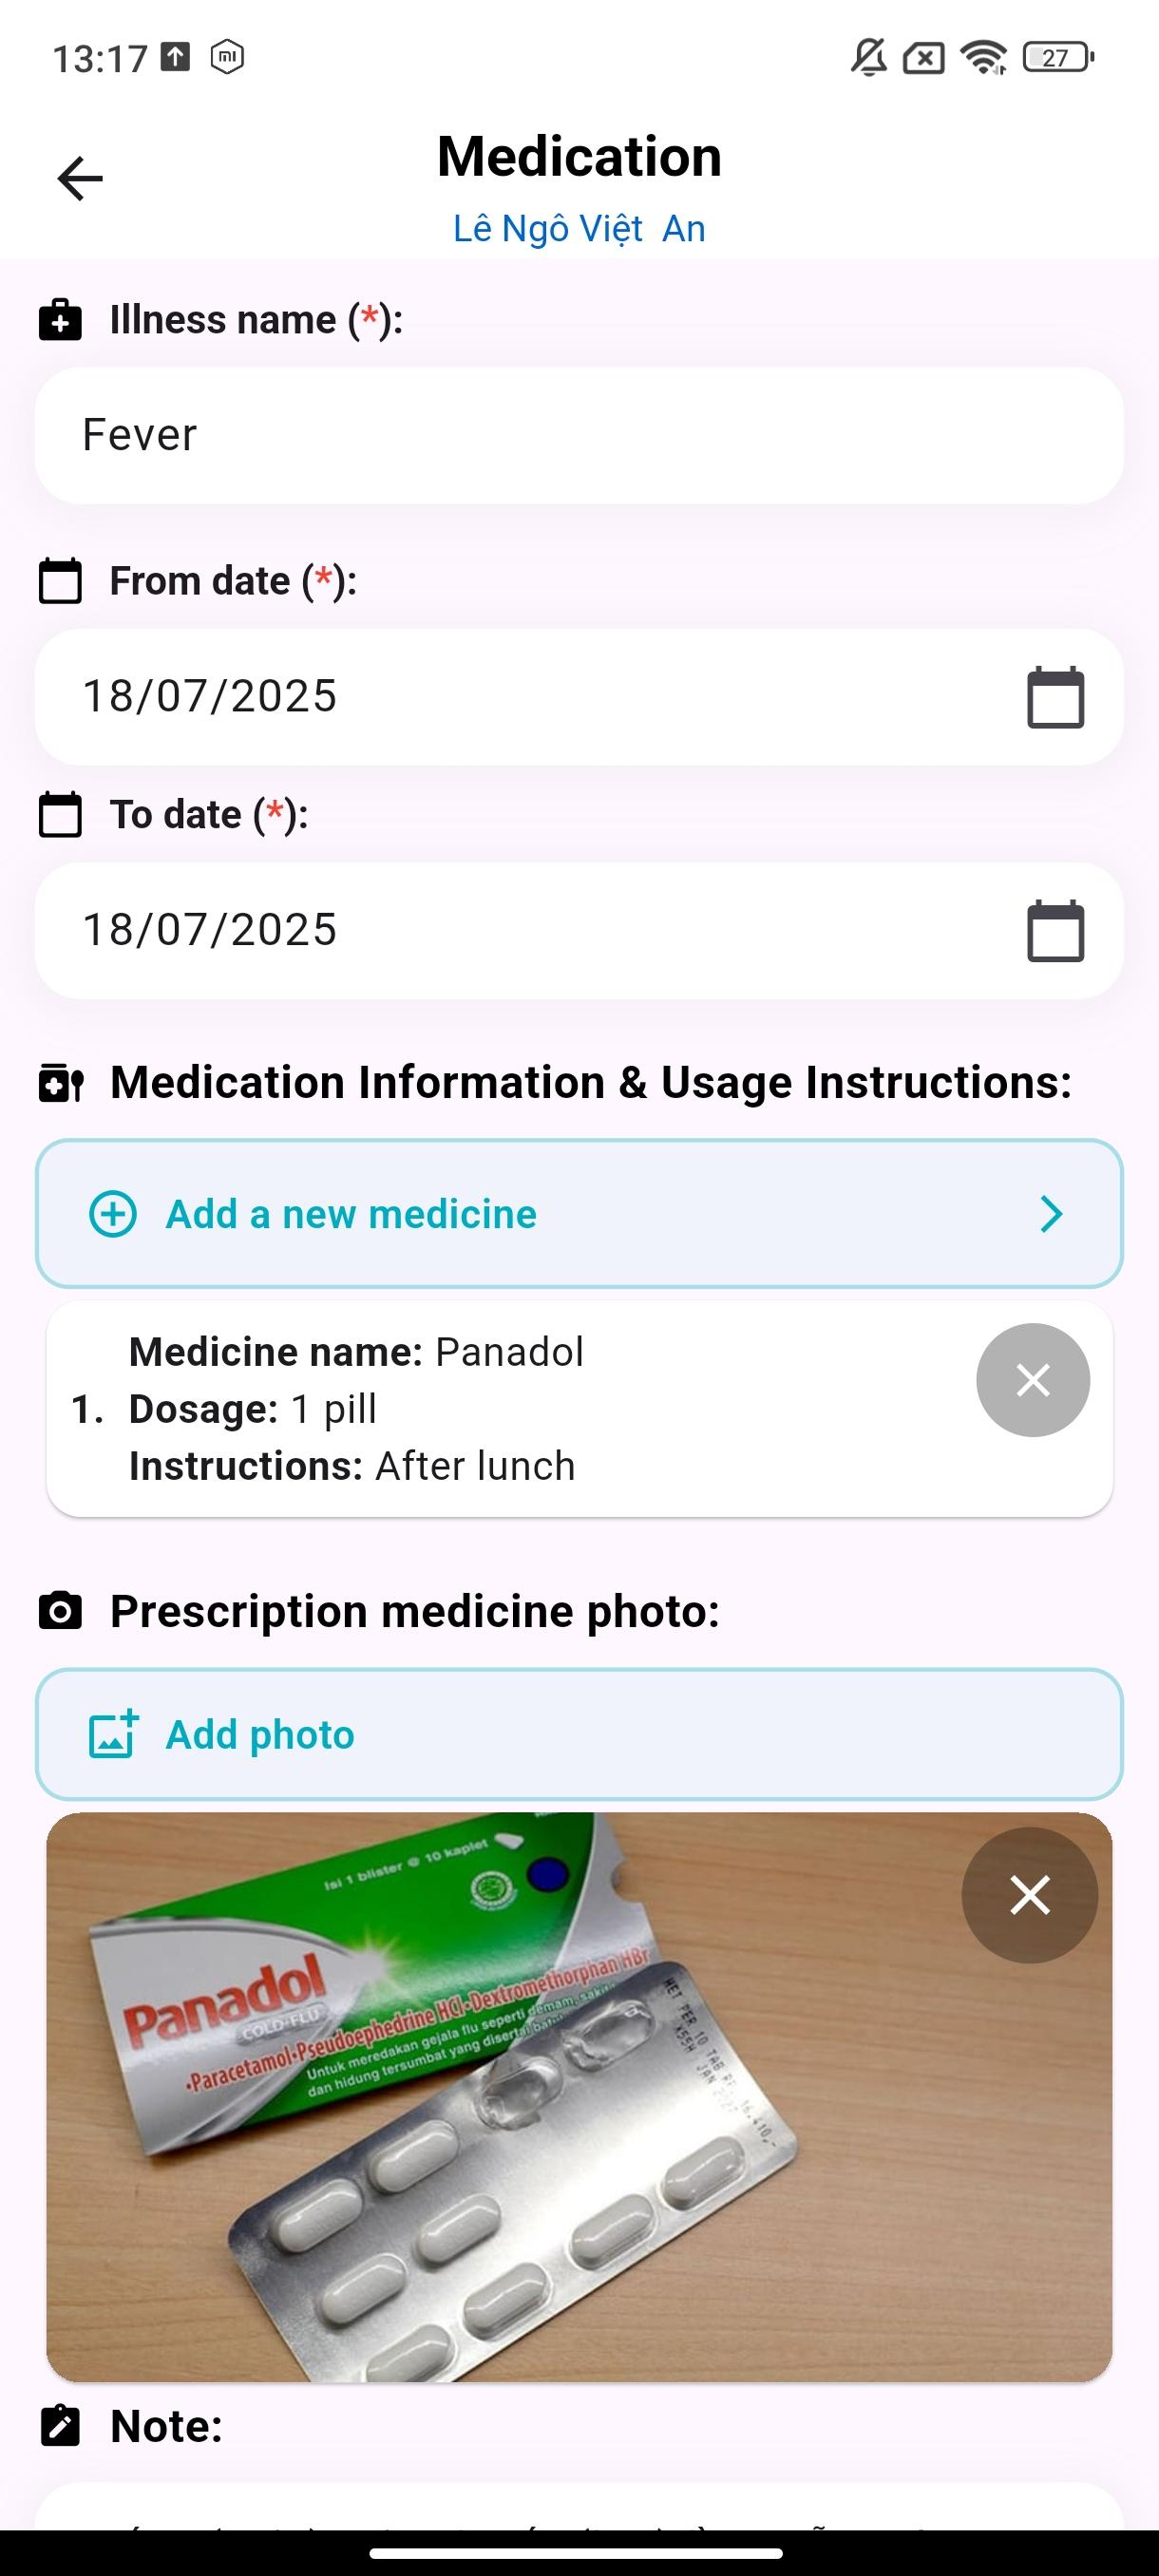
\includegraphics[width=0.6\textwidth]{images/medicine_reminder_parent_view.png}
        \caption{Medicine Reminder - Parent Create View}
        \label{subfig:medicine_reminder_parent_view}
    \end{subfigure}
    \caption{Medicine Reminder mobile app}
    \label{fig:medicine_reminder_mobile_app}
    \end{figure}
    %-----------------
    \item \textbf{Notification Management}
    \begin{figure}[H]
    \centering
    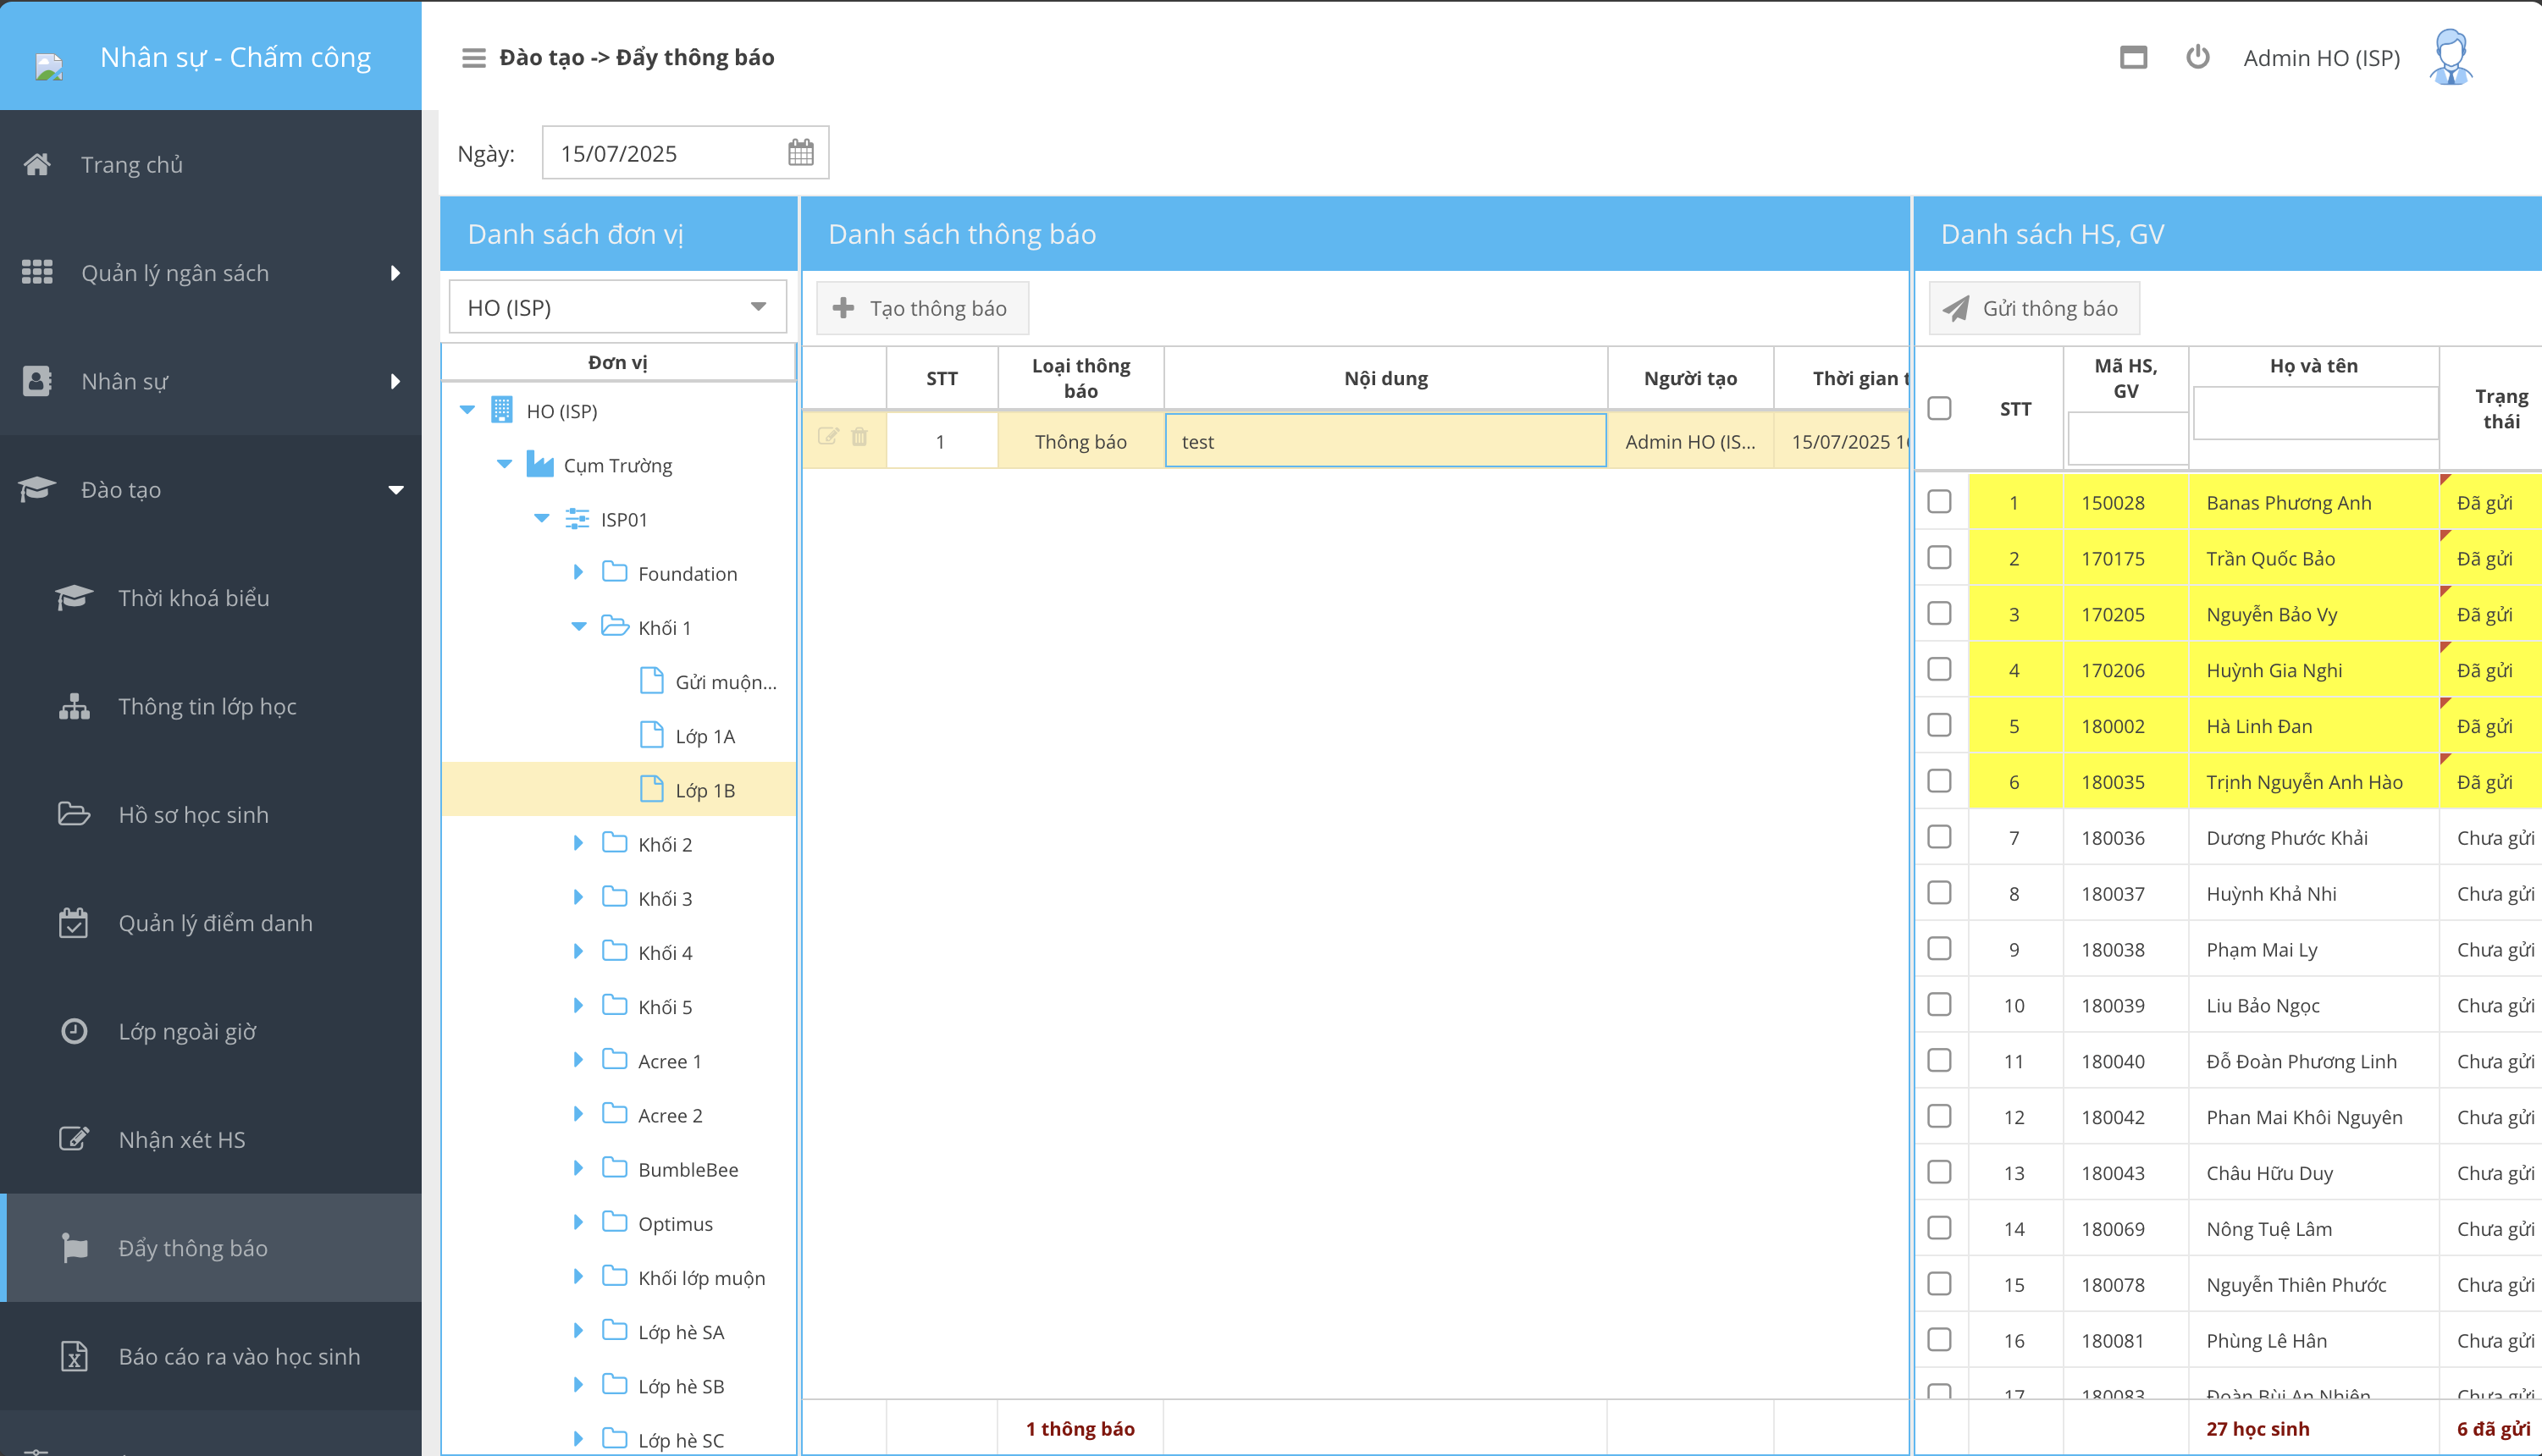
\includegraphics[width=1\textwidth]{images/notification_web.png}
    \vspace{-1em}
    \caption{Push notification web app.}
    \label{fig:push_notification_web}
    \end{figure}
    \begin{figure}[H]
    \centering
    \begin{subfigure}{0.45\textwidth}
        \centering
        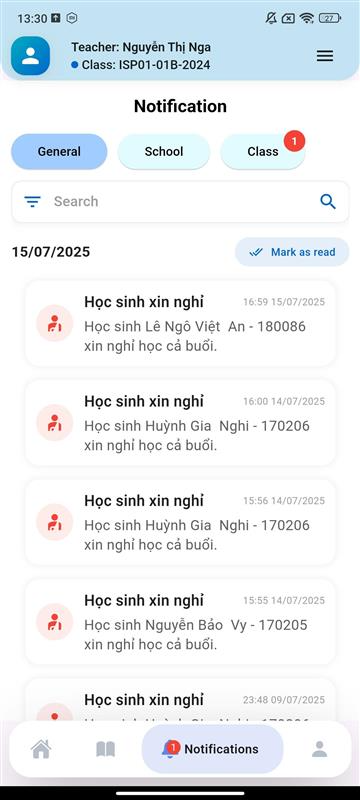
\includegraphics[width=0.6\textwidth]{images/notification_teacher_view.png}
        \caption{Notification - Teacher View}
        \label{subfig:notification_teacher_view}
    \end{subfigure}
    \hfill
    \begin{subfigure}{0.45\textwidth}
        \centering
        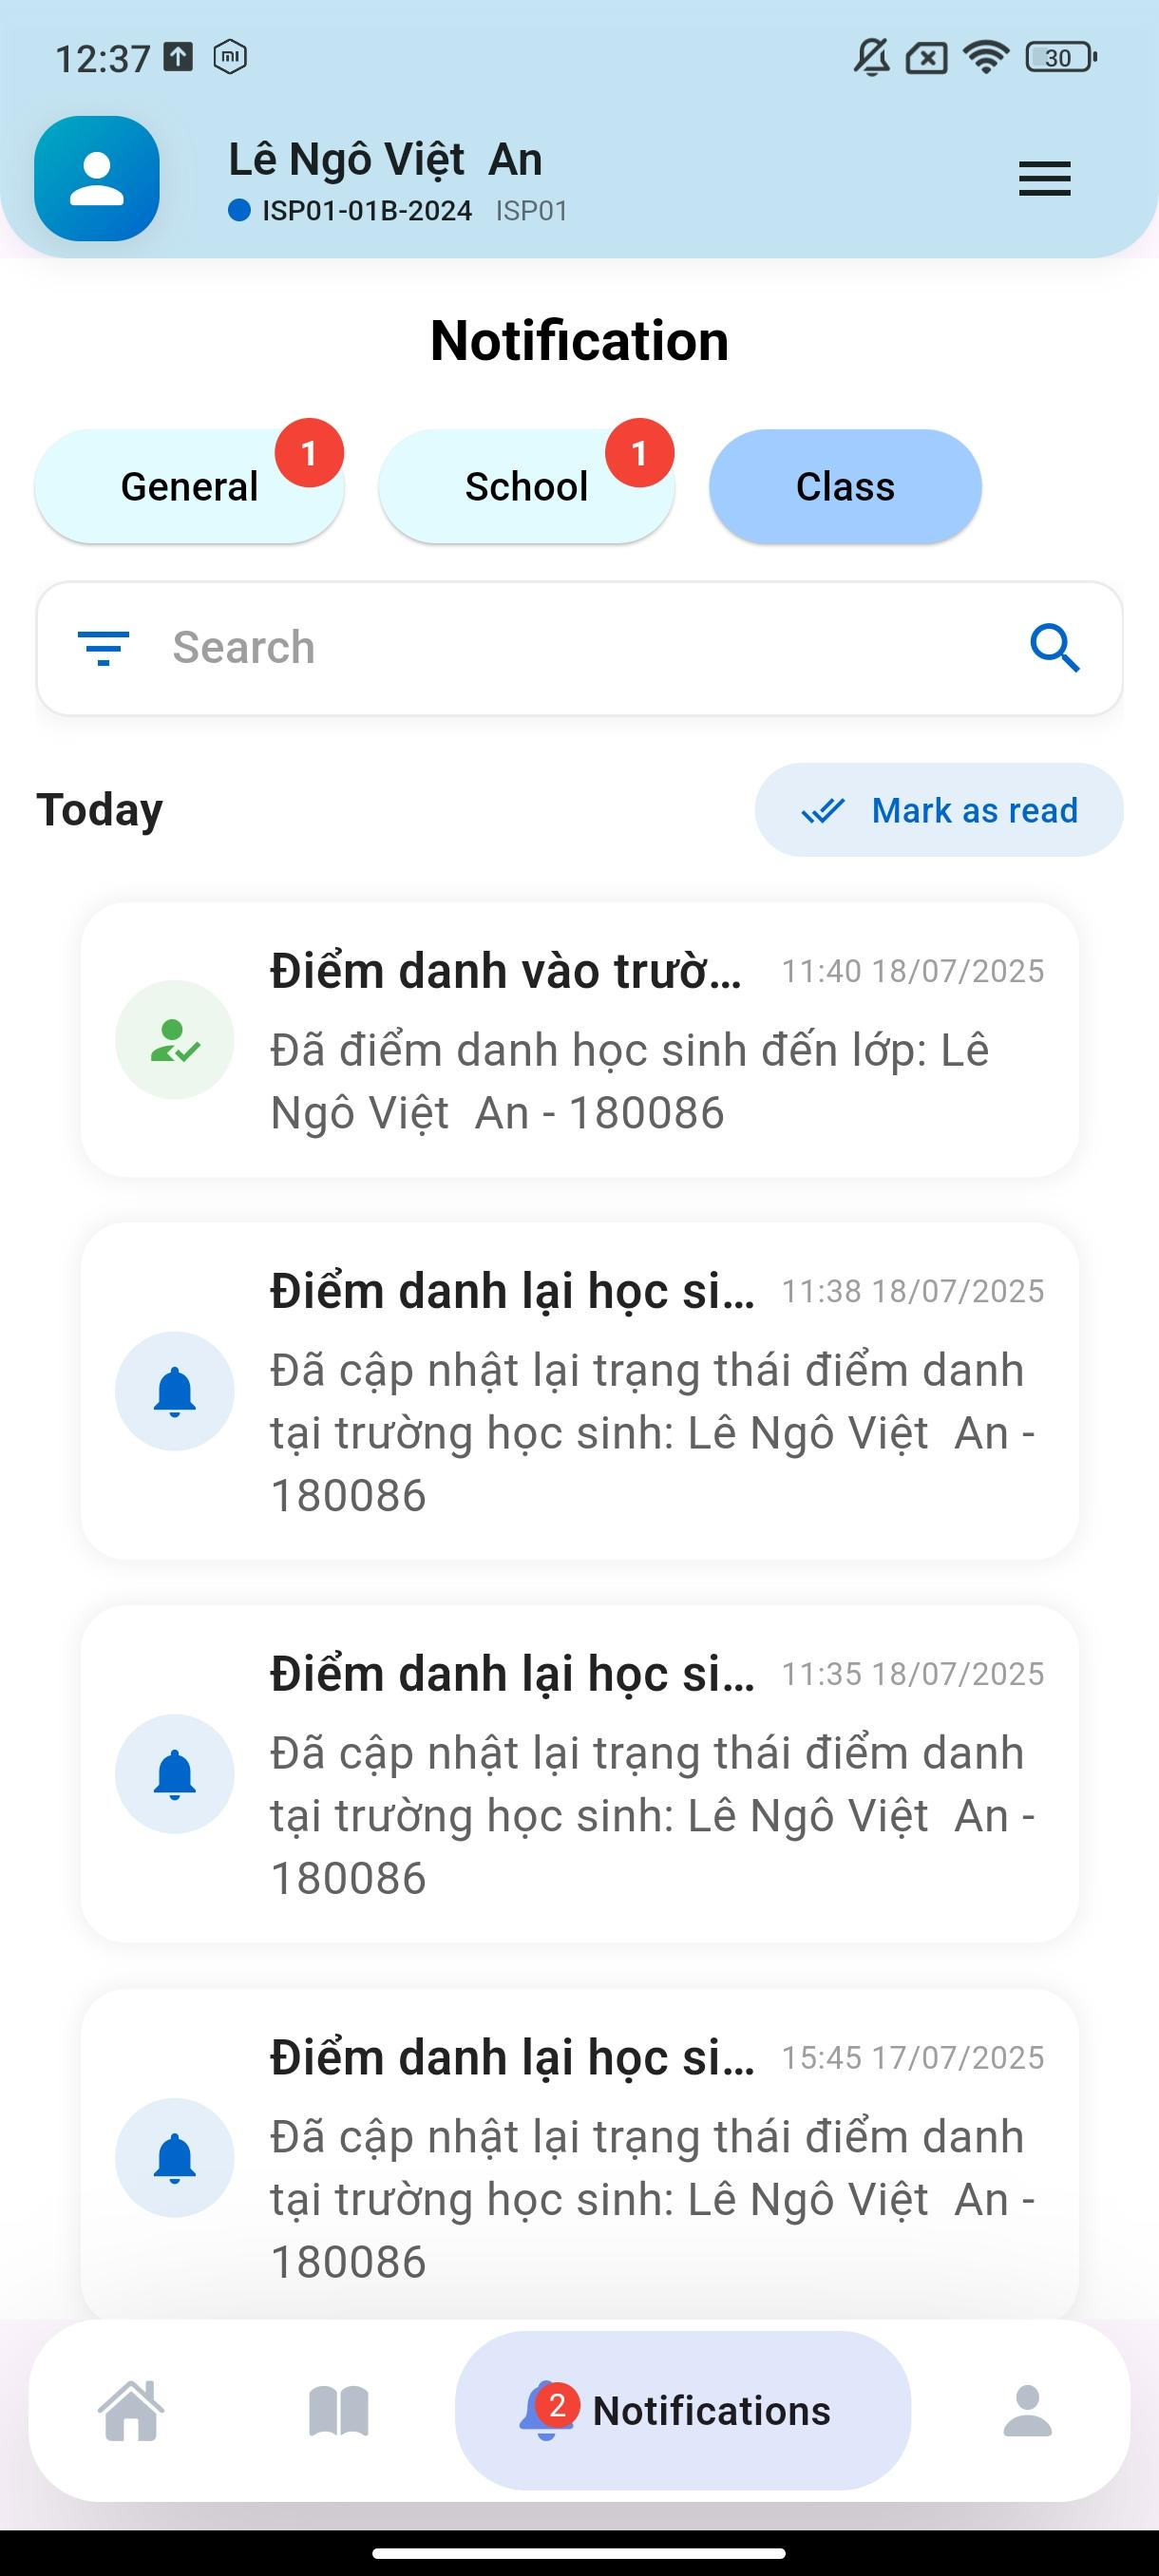
\includegraphics[width=0.6\textwidth]{images/notification_parent_view.png}
        \caption{Notification - Parent Create View}
        \label{subfig:notification_parent_view}
    \end{subfigure}
    \caption{Notification mobile app}
    \label{fig:notification_mobile_app}
    \end{figure}
    %-----------------
    \end{itemize}
\vspace{0.1cm}
\begin{minipage}{\textwidth}
    \setlength{\parindent}{2em}
   Additionally, I have \textbf{implemented and updated some key features} for the system such as:
\end{minipage}
\begin{itemize}[itemsep=-0.05cm, topsep=0.2cm]
    \item \textbf{Import/Export employee and student data}
    \item \textbf{Registering bus stop} (for mobile app)
    \item \textbf{Real-time Bus tracking} (for back-end part not the UI part)
\end{itemize}
\begin{minipage}{\textwidth}
    \setlength{\parindent}{2em}The modules and features I implemented have \textbf{passed almost all business test cases} and have been published for client verification. Additionally, I have \textbf{improved the system's performance} when handling large volumes of data, reducing the load time from minutes to just 3 seconds by \textbf{implementing pagination and multithreading}. Furthermore, the team and I have \textbf{collaborated to successfully publish the mobile application to the App Store and Google Play (CH Play)}, expanding accessibility for end users.
\end{minipage}
\begin{figure}[H]
    \centering
    
\includegraphics[width=0.35\textwidth]{images/ios_pathway.png}
    \caption{Mobile app on iOS}
    \label{subfig:ios_app}
\end{figure}
\begin{figure}[H]
    \centering
    
\includegraphics[width=0.6\textwidth]{images/android_pathway.png}
    \vspace{-1em}
    \caption{Mobile app on Android}
        \label{subfig:android_app}
\end{figure}
